% Options for packages loaded elsewhere
\PassOptionsToPackage{unicode}{hyperref}
\PassOptionsToPackage{hyphens}{url}
\PassOptionsToPackage{dvipsnames,svgnames,x11names}{xcolor}
%
\documentclass[
  letterpaper,
  DIV=11,
  numbers=noendperiod]{scrreprt}

\usepackage{amsmath,amssymb}
\usepackage{lmodern}
\usepackage{iftex}
\ifPDFTeX
  \usepackage[T1]{fontenc}
  \usepackage[utf8]{inputenc}
  \usepackage{textcomp} % provide euro and other symbols
\else % if luatex or xetex
  \usepackage{unicode-math}
  \defaultfontfeatures{Scale=MatchLowercase}
  \defaultfontfeatures[\rmfamily]{Ligatures=TeX,Scale=1}
\fi
% Use upquote if available, for straight quotes in verbatim environments
\IfFileExists{upquote.sty}{\usepackage{upquote}}{}
\IfFileExists{microtype.sty}{% use microtype if available
  \usepackage[]{microtype}
  \UseMicrotypeSet[protrusion]{basicmath} % disable protrusion for tt fonts
}{}
\makeatletter
\@ifundefined{KOMAClassName}{% if non-KOMA class
  \IfFileExists{parskip.sty}{%
    \usepackage{parskip}
  }{% else
    \setlength{\parindent}{0pt}
    \setlength{\parskip}{6pt plus 2pt minus 1pt}}
}{% if KOMA class
  \KOMAoptions{parskip=half}}
\makeatother
\usepackage{xcolor}
\setlength{\emergencystretch}{3em} % prevent overfull lines
\setcounter{secnumdepth}{5}
% Make \paragraph and \subparagraph free-standing
\ifx\paragraph\undefined\else
  \let\oldparagraph\paragraph
  \renewcommand{\paragraph}[1]{\oldparagraph{#1}\mbox{}}
\fi
\ifx\subparagraph\undefined\else
  \let\oldsubparagraph\subparagraph
  \renewcommand{\subparagraph}[1]{\oldsubparagraph{#1}\mbox{}}
\fi


\providecommand{\tightlist}{%
  \setlength{\itemsep}{0pt}\setlength{\parskip}{0pt}}\usepackage{longtable,booktabs,array}
\usepackage{calc} % for calculating minipage widths
% Correct order of tables after \paragraph or \subparagraph
\usepackage{etoolbox}
\makeatletter
\patchcmd\longtable{\par}{\if@noskipsec\mbox{}\fi\par}{}{}
\makeatother
% Allow footnotes in longtable head/foot
\IfFileExists{footnotehyper.sty}{\usepackage{footnotehyper}}{\usepackage{footnote}}
\makesavenoteenv{longtable}
\usepackage{graphicx}
\makeatletter
\def\maxwidth{\ifdim\Gin@nat@width>\linewidth\linewidth\else\Gin@nat@width\fi}
\def\maxheight{\ifdim\Gin@nat@height>\textheight\textheight\else\Gin@nat@height\fi}
\makeatother
% Scale images if necessary, so that they will not overflow the page
% margins by default, and it is still possible to overwrite the defaults
% using explicit options in \includegraphics[width, height, ...]{}
\setkeys{Gin}{width=\maxwidth,height=\maxheight,keepaspectratio}
% Set default figure placement to htbp
\makeatletter
\def\fps@figure{htbp}
\makeatother
\newlength{\cslhangindent}
\setlength{\cslhangindent}{1.5em}
\newlength{\csllabelwidth}
\setlength{\csllabelwidth}{3em}
\newlength{\cslentryspacingunit} % times entry-spacing
\setlength{\cslentryspacingunit}{\parskip}
\newenvironment{CSLReferences}[2] % #1 hanging-ident, #2 entry spacing
 {% don't indent paragraphs
  \setlength{\parindent}{0pt}
  % turn on hanging indent if param 1 is 1
  \ifodd #1
  \let\oldpar\par
  \def\par{\hangindent=\cslhangindent\oldpar}
  \fi
  % set entry spacing
  \setlength{\parskip}{#2\cslentryspacingunit}
 }%
 {}
\usepackage{calc}
\newcommand{\CSLBlock}[1]{#1\hfill\break}
\newcommand{\CSLLeftMargin}[1]{\parbox[t]{\csllabelwidth}{#1}}
\newcommand{\CSLRightInline}[1]{\parbox[t]{\linewidth - \csllabelwidth}{#1}\break}
\newcommand{\CSLIndent}[1]{\hspace{\cslhangindent}#1}

\KOMAoption{captions}{tableheading}
\makeatletter
\makeatother
\makeatletter
\@ifpackageloaded{bookmark}{}{\usepackage{bookmark}}
\makeatother
\makeatletter
\@ifpackageloaded{caption}{}{\usepackage{caption}}
\AtBeginDocument{%
\ifdefined\contentsname
  \renewcommand*\contentsname{Table of contents}
\else
  \newcommand\contentsname{Table of contents}
\fi
\ifdefined\listfigurename
  \renewcommand*\listfigurename{List of Figures}
\else
  \newcommand\listfigurename{List of Figures}
\fi
\ifdefined\listtablename
  \renewcommand*\listtablename{List of Tables}
\else
  \newcommand\listtablename{List of Tables}
\fi
\ifdefined\figurename
  \renewcommand*\figurename{Figure}
\else
  \newcommand\figurename{Figure}
\fi
\ifdefined\tablename
  \renewcommand*\tablename{Table}
\else
  \newcommand\tablename{Table}
\fi
}
\@ifpackageloaded{float}{}{\usepackage{float}}
\floatstyle{ruled}
\@ifundefined{c@chapter}{\newfloat{codelisting}{h}{lop}}{\newfloat{codelisting}{h}{lop}[chapter]}
\floatname{codelisting}{Listing}
\newcommand*\listoflistings{\listof{codelisting}{List of Listings}}
\makeatother
\makeatletter
\@ifpackageloaded{caption}{}{\usepackage{caption}}
\@ifpackageloaded{subcaption}{}{\usepackage{subcaption}}
\makeatother
\makeatletter
\@ifpackageloaded{tcolorbox}{}{\usepackage[many]{tcolorbox}}
\makeatother
\makeatletter
\@ifundefined{shadecolor}{\definecolor{shadecolor}{rgb}{.97, .97, .97}}
\makeatother
\makeatletter
\makeatother
\ifLuaTeX
  \usepackage{selnolig}  % disable illegal ligatures
\fi
\IfFileExists{bookmark.sty}{\usepackage{bookmark}}{\usepackage{hyperref}}
\IfFileExists{xurl.sty}{\usepackage{xurl}}{} % add URL line breaks if available
\urlstyle{same} % disable monospaced font for URLs
\hypersetup{
  pdftitle={pkpd notes},
  pdfauthor={Nazmul Alam},
  colorlinks=true,
  linkcolor={blue},
  filecolor={Maroon},
  citecolor={Blue},
  urlcolor={Blue},
  pdfcreator={LaTeX via pandoc}}

\title{pkpd notes}
\author{Nazmul Alam}
\date{2/6/23}

\begin{document}
\maketitle
\ifdefined\Shaded\renewenvironment{Shaded}{\begin{tcolorbox}[boxrule=0pt, breakable, interior hidden, borderline west={3pt}{0pt}{shadecolor}, sharp corners, enhanced, frame hidden]}{\end{tcolorbox}}\fi

\renewcommand*\contentsname{Table of contents}
{
\hypersetup{linkcolor=}
\setcounter{tocdepth}{2}
\tableofcontents
}
\bookmarksetup{startatroot}

\hypertarget{preface}{%
\chapter*{Preface}\label{preface}}
\addcontentsline{toc}{chapter}{Preface}

\markboth{Preface}{Preface}

This page is from index page

\bookmarksetup{startatroot}

\hypertarget{introduction-to-winnonlin-122-d}{%
\chapter{Introduction to WinNonlin
(122-D)}\label{introduction-to-winnonlin-122-d}}

\hypertarget{project-setup}{%
\section{Project setup}\label{project-setup}}

\begin{enumerate}
\def\labelenumi{\arabic{enumi}.}
\tightlist
\item
  Create Project
\end{enumerate}

Phenoex Projects

\begin{itemize}
\item
  contains all the data and calculations
\item
  multiple projects can be open at the same time
\item
  common data file to import: excel, csv
\item
  older version can always be opened by newer version
\item
  newer version projects can not be opened by older ones
\item
  Create a project
\item
  Click to history tab to see the project history
\item
  Click to properties tab, where most of the work is done
\end{itemize}

\begin{enumerate}
\def\labelenumi{\arabic{enumi}.}
\setcounter{enumi}{1}
\tightlist
\item
  Create Worksheets
\end{enumerate}

\begin{itemize}
\tightlist
\item
  Right click on Data, select New, select Worksheet
\item
  Add columns, give column name, assign data type
\item
  assign units: select time from list of columns, click Unit Builder
  button, specify h to the time, click Add button,click OK
\item
  for dose, specify mass prefex, click Add
\item
  Type numbers on the worksheet to add values to the cells
\end{itemize}

\begin{enumerate}
\def\labelenumi{\arabic{enumi}.}
\setcounter{enumi}{2}
\tightlist
\item
  Import Files
\end{enumerate}

\begin{itemize}
\tightlist
\item
  file type: xls, xlsx, csv, SAS
\item
  typical data file contains header and unit row.
\item
  Select the Import button, select the file
\item
  on the File import wizard, select appropriate options
\item
  Preview area helps to see the changes
\item
  If units are in the column header, select ``has units in the header''
\end{itemize}

Excels with multiple worksheet:

\begin{itemize}
\tightlist
\item
  click the arrow to move on the Wizard to the next worksheet
\end{itemize}

\begin{enumerate}
\def\labelenumi{\arabic{enumi}.}
\setcounter{enumi}{3}
\tightlist
\item
  Save Projects
\end{enumerate}

\begin{itemize}
\tightlist
\item
  Click the save icon on the toolbar
\item
  File name can be completely different from the Project name
\item
  No auto-save options
\item
  sharing project file will also share the embedded data files
\item
  Close project by right clicking the project name
\item
  After opening a saved project folder, expand the plus sign to see the
  contents.
\end{itemize}

\begin{enumerate}
\def\labelenumi{\arabic{enumi}.}
\setcounter{enumi}{4}
\tightlist
\item
  Set Project Preferences
\end{enumerate}

\begin{itemize}
\tightlist
\item
  Select the Edit menu -\textgreater{} preferences -\textgreater{}
  Projects
\item
  Check Autosave on execution
\item
  update the save locations and hit apply before clicking on OK.
\end{itemize}

\hypertarget{create-and-modify-worksheets}{%
\section{Create and Modify
Worksheets}\label{create-and-modify-worksheets}}

\begin{enumerate}
\def\labelenumi{\arabic{enumi}.}
\tightlist
\item
  Sort Rows
\end{enumerate}

\begin{itemize}
\tightlist
\item
  data can be sorted by subject, dose level,
\item
  sort button on every worksheet
\item
  Use the ``sort worksheet'' window to apply sort options
\end{itemize}

\begin{enumerate}
\def\labelenumi{\arabic{enumi}.}
\setcounter{enumi}{1}
\tightlist
\item
  Move Columns
\end{enumerate}

\begin{itemize}
\tightlist
\item
  Select a column from the column list
\item
  Click the up or down arrow to move
\end{itemize}

\begin{enumerate}
\def\labelenumi{\arabic{enumi}.}
\setcounter{enumi}{2}
\tightlist
\item
  Rename Columns
\end{enumerate}

\begin{itemize}
\tightlist
\item
  Click the column name, type F2 or double click on it to edit the name
\end{itemize}

\begin{enumerate}
\def\labelenumi{\arabic{enumi}.}
\setcounter{enumi}{3}
\tightlist
\item
  Apply Units
\end{enumerate}

\begin{itemize}
\tightlist
\item
  Select column
\item
  Click the Unit Builder
\item
  Click Clear Units
\item
  Add units
\end{itemize}

\begin{enumerate}
\def\labelenumi{\arabic{enumi}.}
\setcounter{enumi}{4}
\tightlist
\item
  Convert Units
\end{enumerate}

\begin{itemize}
\tightlist
\item
  convert amount column from microgram to miligram
\item
  click the Amount column
\item
  type mg in the New unit box,click OK
\item
  To convert ng/mL to nmole/mL, add nmol and then click the slash
  button, specify the volume unit, enter molecular weight, click OK.
\item
  Better way: use the Data Wizard to convert the units.
\end{itemize}

\hypertarget{plot-data}{%
\section{Plot Data}\label{plot-data}}

\begin{enumerate}
\def\labelenumi{\arabic{enumi}.}
\tightlist
\item
  Create Simple Plot
\end{enumerate}

\begin{itemize}
\tightlist
\item
  Data: Conc, Time, dose level: 16 mg, 10 subjects
\item
  right click the worksheet
\item
  Select send to -\textgreater{} plotting -\textgreater{} xy plot
\item
  XY object is created with the linked data source
\item
  On the mapping window, orange column headers are required mappings
\item
  map, x -\textgreater{} Time, y -\textgreater{} conc, Group
  -\textgreater{} subject
\item
  click execute
\item
  Options pan - Axes - Y - select log button
\item
  Options pan - Graphs - rename by typing F2
\item
  Graph name and legend names are the same
\end{itemize}

\begin{enumerate}
\def\labelenumi{\arabic{enumi}.}
\setcounter{enumi}{1}
\tightlist
\item
  Create Lattice Plot
\end{enumerate}

\begin{itemize}
\tightlist
\item
  Data: Conc, Time, Administration, dose level 4 mg for IV, 8 mg for PO,
  10 subjects
\item
  Create a XY plot object same as above
\item
  map x - Time, y - conc, group - subject, lattice column -
  administration
\item
  Execute and get two plots
\item
  Options - range - `auto scale best' settings scales individual plots
  are independent
\end{itemize}

\begin{enumerate}
\def\labelenumi{\arabic{enumi}.}
\setcounter{enumi}{2}
\tightlist
\item
  Use Second Y Axis
\end{enumerate}

\begin{itemize}
\tightlist
\item
  Data: plasma conc, urine conc, time, 10 subjects
\item
  Creat XY plot object same as above
\item
  map x - Time, y - plasma conc, y2 - urine conc, lattice condition,
  page (sort) - Subject
\item
  plots are on a single page for each subject
\item
  Options - select plasma\_conc vs Time, type F2, change the name to
  Plasma, do the same for Urine
\item
  Execute
\end{itemize}

\begin{enumerate}
\def\labelenumi{\arabic{enumi}.}
\setcounter{enumi}{3}
\tightlist
\item
  Compute Descriptive Statistics
\end{enumerate}

\begin{itemize}
\tightlist
\item
  Needed to create a plot with mean and error bars
\item
  right click on data sheet, send to - computation tools - Discriptive
  statistics
\item
  map summary - conc, sort - Time
\item
  Execute
\item
  Options pannel - click Clear All - click basic statistics, check Mean
  and SD
\end{itemize}

\begin{enumerate}
\def\labelenumi{\arabic{enumi}.}
\setcounter{enumi}{4}
\tightlist
\item
  Use Error Bars
\end{enumerate}

\begin{itemize}
\tightlist
\item
  Discriptive Satistics object - Output data - right click on Statistics
\item
  send to plotting - XY plot
\item
  map x - Time, y - Mean, Error bars, lower - SD, Error bars, upper - SD
\item
  Execute
\item
  set Y axis to log scale
\end{itemize}

\begin{enumerate}
\def\labelenumi{\arabic{enumi}.}
\setcounter{enumi}{5}
\tightlist
\item
  Create Overlay Plot
\end{enumerate}

\begin{itemize}
\item
  duplicate the error bars plot from previous section
\item
  Options pan - Plot - Graphs tab - click Add button
\item
  Select the new second input from the setup tab
\item
  Link the source data by clicking source button,
\item
  map x - Time, y - conc, group - subject
\item
  Execute
\item
  Options pan - select Conc vs Time plot
\item
  Select Quick Styles
\item
  Uncheck Group by lines, uncheck Gourp by colors,
\item
  Select Apprance tab
\item
  Specify color to Silver
\item
  Uncheck Markers visible
\item
  Now all the individual lines are silver color
\item
  Select Mean vs Time graph
\item
  Select Appearance, specify line colors to red, Marker border color -
  red, line weight 3
\item
  Under the Mean vs Time graph, select the Error bars
\item
  Select Appearance, color - red
\item
  Options pan - select Y axis - select Axis label and update
\item
  Options pan - select Legend - uncheck Visible
\end{itemize}

\begin{enumerate}
\def\labelenumi{\arabic{enumi}.}
\setcounter{enumi}{6}
\tightlist
\item
  Create Box Plot
\end{enumerate}

\begin{figure}

{\centering 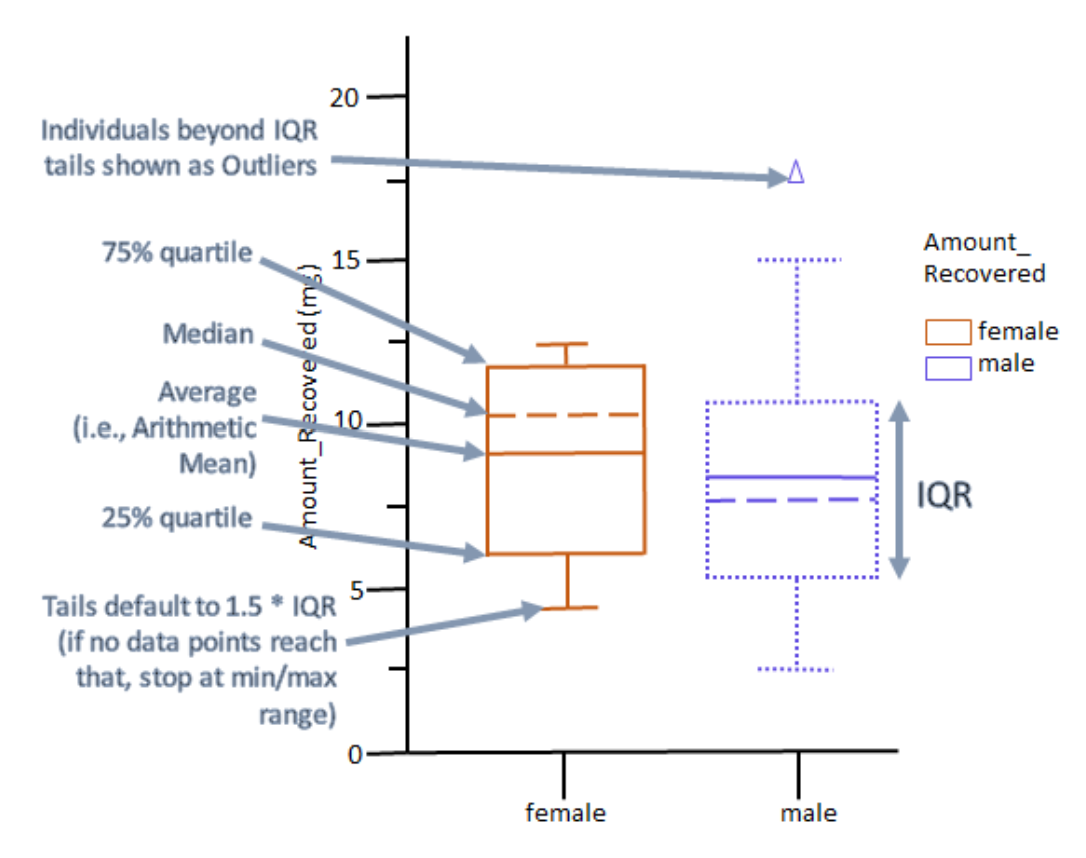
\includegraphics[width=4.5625in,height=\textheight]{./images/image-40592419.png}

}

\end{figure}

\begin{itemize}
\tightlist
\item
  20 subjects, AR: accumulation ratio (how much accumulated under
  repeated ss), dose level, 2 mg and 4 mg
\item
  Is AR increases with increasing dose level?
\item
  right click data, send to - plotting - box plot
\item
  map y - AR, group - dose level
\item
  Execute
\end{itemize}

\begin{enumerate}
\def\labelenumi{\arabic{enumi}.}
\setcounter{enumi}{7}
\tightlist
\item
  Create Plot with Categorical X Axis
\end{enumerate}

\begin{itemize}
\tightlist
\item
  Data: Severity (Mild, Moderate), dose level (1, 2, 4, 8, 16, 32 mg),
  frequency (numerical, i.e., 0, 0.2, 0.6)
\item
  right click the data sheet, send to plotting - X-categorical XY plot
\item
  map x - severity, y - frequency, group - dose level
\item
  Options pan, select X axis, select Order tab, change order if needed
\item
  Options pan - Frequency vs Severity graph - check line visible - now
  points are connected by a line
\end{itemize}

\begin{enumerate}
\def\labelenumi{\arabic{enumi}.}
\setcounter{enumi}{8}
\tightlist
\item
  Set Plot Preferences
\end{enumerate}

\begin{itemize}
\tightlist
\item
  Options pan - Plot - Layout
  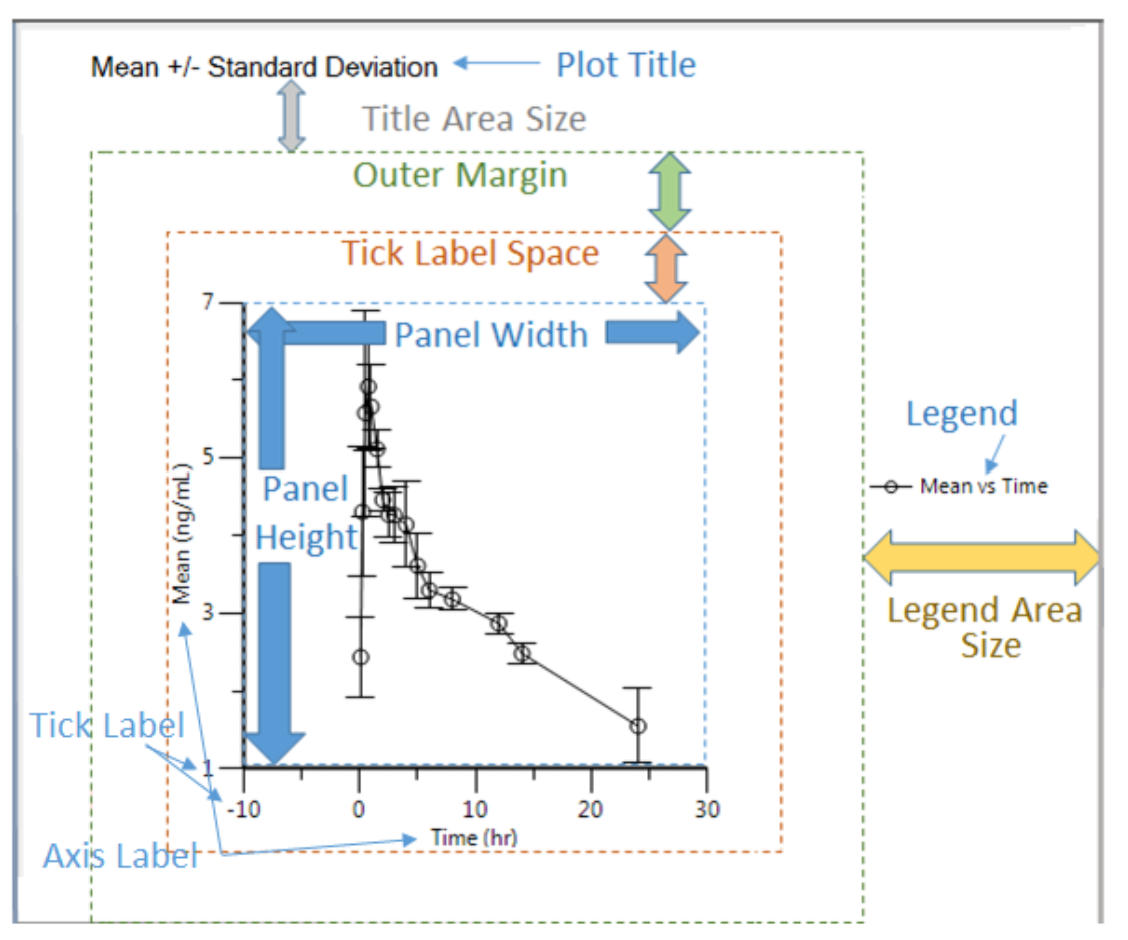
\includegraphics[width=4.15625in,height=\textheight]{./images/image-1684060613.png}
\item
  Edit menu bar, preferences, plotting details
\item
  Changing prefernences affect all new plots
\end{itemize}

\hypertarget{introduction-to-nca}{%
\section{Introduction to NCA}\label{introduction-to-nca}}

\hypertarget{about-nca}{%
\subsection{About NCA}\label{about-nca}}

Non-compartmental analysis or NCA is a method for quantifying drug
exposure

\begin{itemize}
\item
  NCA determines a large number of pharmacokinetic descriptors or PK
  parameters for a drug
\item
  They are not really parameters as you would have in a model
\item
  NCA does not use any kind of model other than assuming that the
  elimination can be described by first order kinetics
\item
  because there is no model at the heart of the method we cannot really
  use it for predictions
\item
  An example plot of concentration over time following an extravascular
  dose NCA will give us two different measures of drug exposure:

  \begin{itemize}
  \item
    the peak exposure to the drug concentration occurring after dosing
  \item
    The overall exposure is measured by computing the area under the
    curve or AUC
  \item
    an extra vascular dose starts with a concentration of zero, the
    concentration rises rapidly reaches C\textsubscript{max} and then
    decreases

    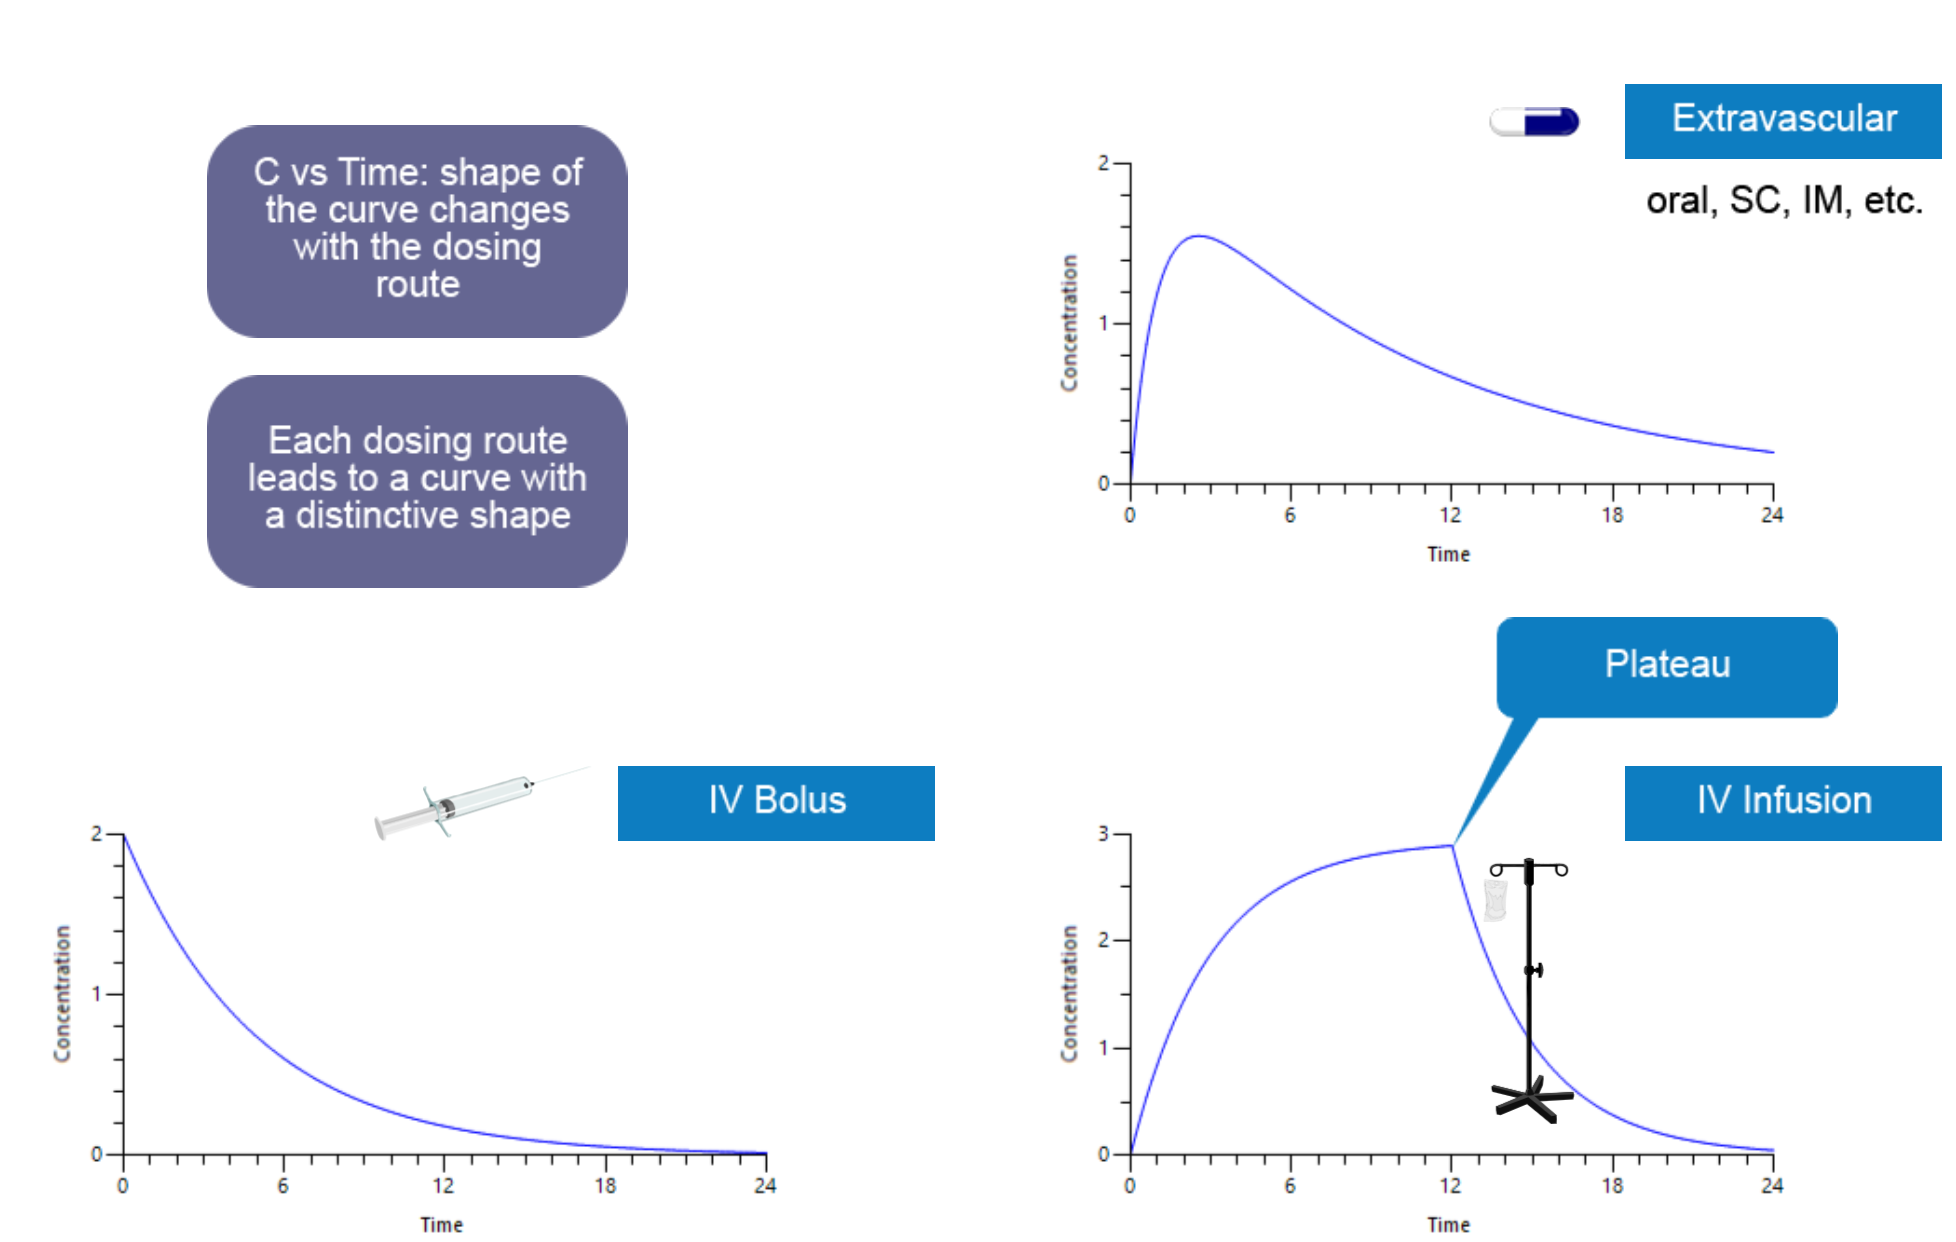
\includegraphics[width=5.79167in,height=\textheight]{./images/image-1998985080.png}
  \end{itemize}
\item
  with extra vascular dosing there is an absorption process that leads
  to a maximum concentration followed by elimination
\item
  IV bolus dosing: drug is directly injected all at once into a vein;
  the mixing and systemic circulation is very fast and by the time the
  first sample is taken after dosing the mixing is assumed to be
  complete. The concentration starts high and then decreases as the drug
  is eliminated.
\item
  IV infusion: the concentration starts at zero and then rises if the
  infusion is continued for long enough the concentration approaches a
  plateau at steady state when the infusion stops the concentration then
  falls in the same manner as in ivy bolus dosing
\item
  plotting on a log scale is useful because it usually shows linear
  elimination in each case regardless of the dosing root we could fit
  the linear portion with a straight line to predict what will happen to
  concentration after we've collected the last sample concentration on
  the log axis
\end{itemize}

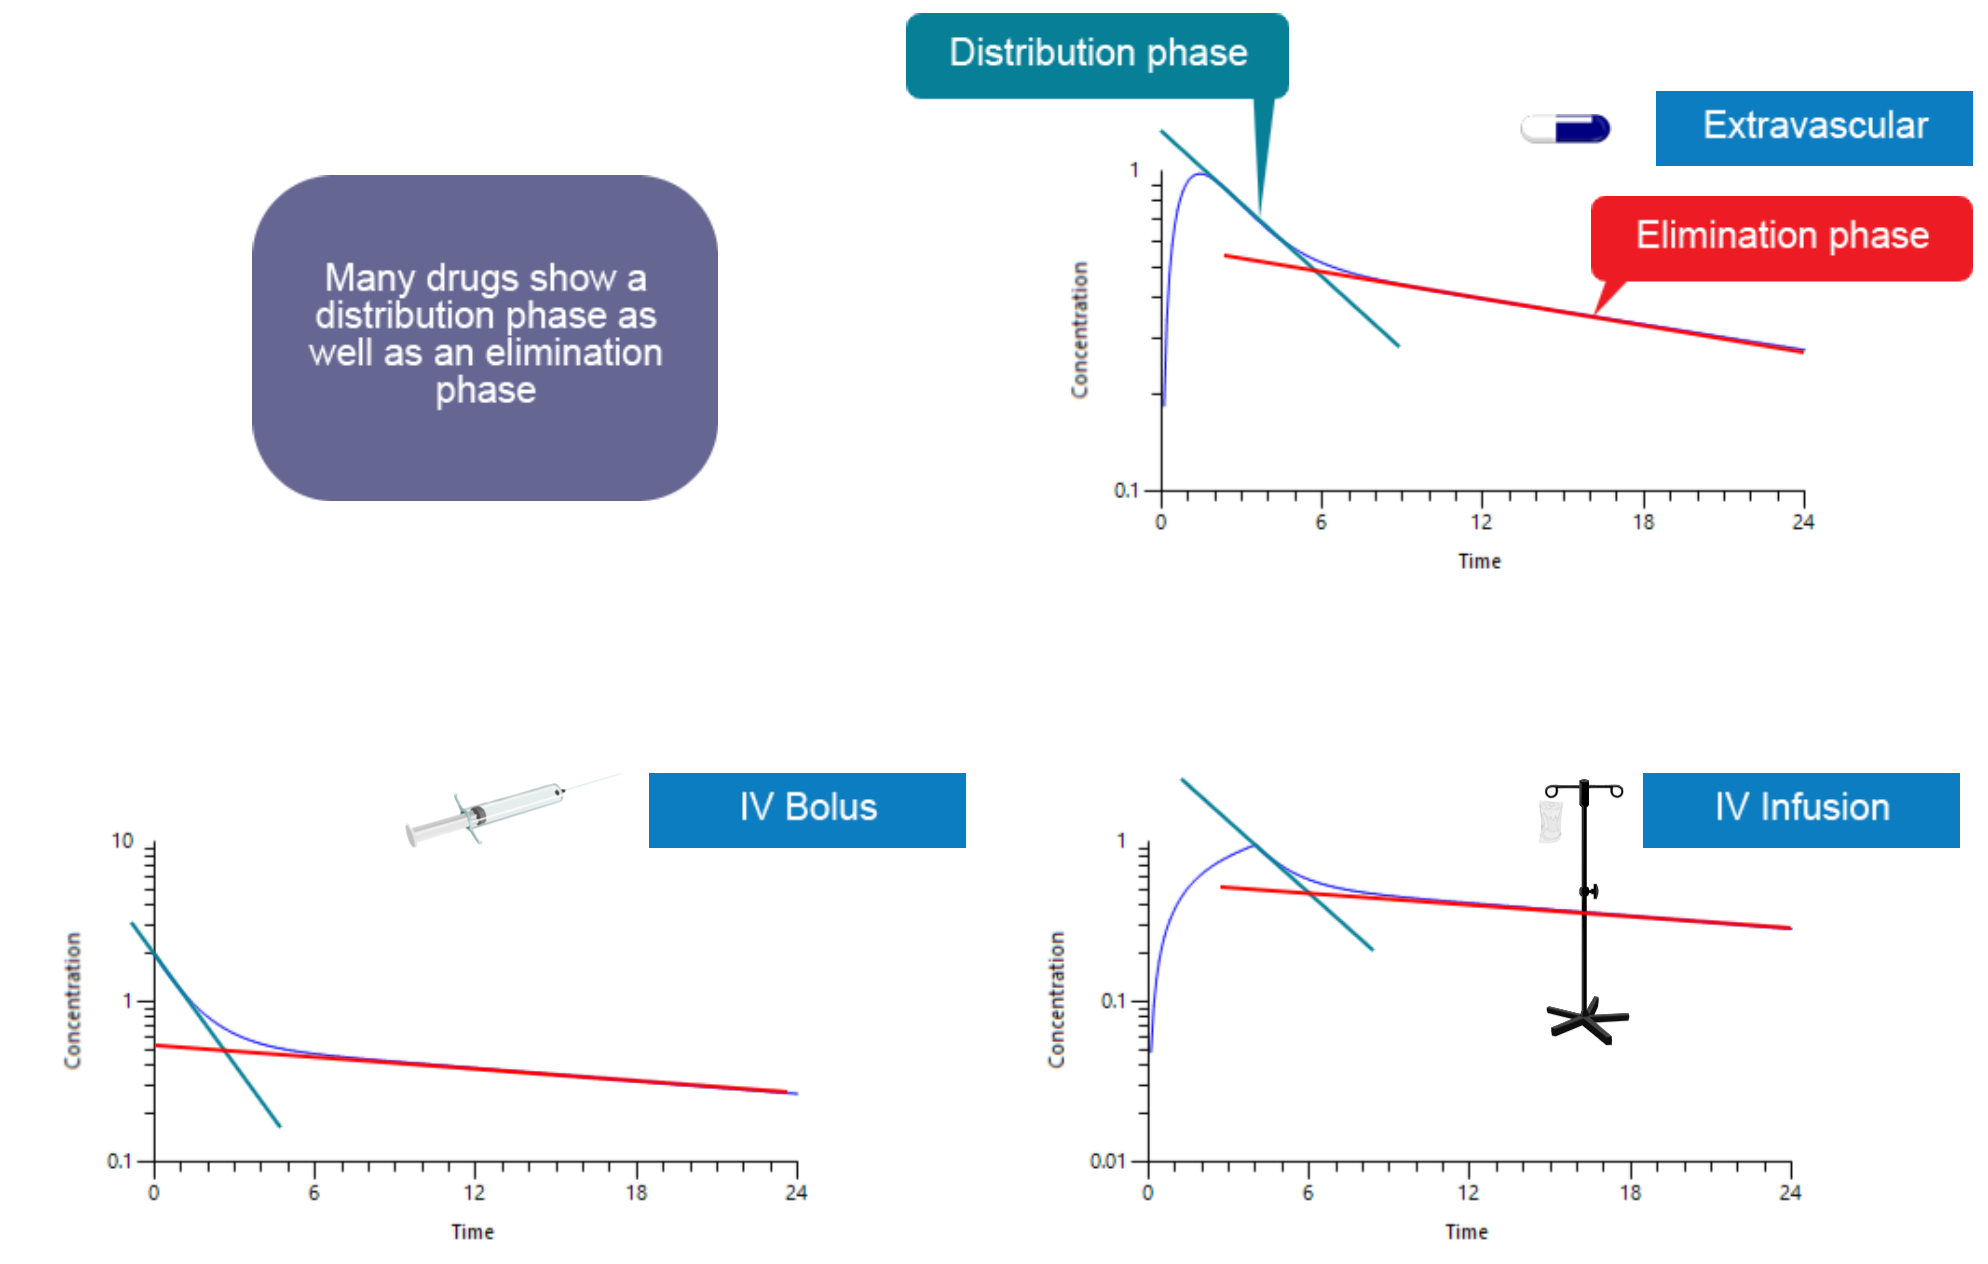
\includegraphics[width=6.11458in,height=\textheight]{./images/image-781344710.png}

\begin{itemize}
\item
  It is useful to have both linear and log plots. Linear plots are
  useful for examining the peak concentration and log plots are useful
  for the low concentrations
\item
  In addition to an elimination phase many drugs also show a
  distribution phase in such cases there may be two distinctive straight
  line sections on the plot. Although sometimes the two phases blend
  into a general curvature in the plots we see here the distribution
  phase is apparent for all three dosing routs but it is most pronounced
  for the IV bolus dosing. For extravascular dosing the distribution
  phase may be obscured by the drug absorption.
\item
  The AUC can be determined no matter how complex the relationship
  between concentration and time.

  Summary:
\item
  NCA is the primary method of assessing drug exposure.
\item
  C\textsubscript{max} is a measure of peak exposure
\item
  AUC is a measure of the overall exposure to the drug
\item
  different dosing route leads to a curve with the distinctive shape
  that plotting on a log concentration scale usually shows linear
  elimination
\item
  many drugs show a distribution phase as well as an elimination phase\\
\end{itemize}

\hypertarget{observe-parameters}{%
\subsection{Observe Parameters}\label{observe-parameters}}

\begin{itemize}
\tightlist
\item
  From the plot of concentration versus time, we can see that the
  maximum concentration is reached at about 1 hour, we call that time
  T\textsubscript{max} and the concentration at the peak is
  C\textsubscript{max}
\item
  T\textsubscript{max} and C\textsubscript{max} are listed in the output
  of NCA in Phoenix
\item
  At some point after dosing we will have our last observed
  concentration this may be because we have stopped collecting samples
  or the concentration may have dropped below the quantification limit
  for the analysis and therefore we were unable to get more values The
  point is at a time of t last and has a concentration of
  T\textsubscript{last} These observeed parameters are affected by the
  sampling schedule we can improve our chances by sampling richly around
  the expected time of c max if we have more points we have a better
  chance of capturing a concentration that is near the true maximum
\end{itemize}

Summarize

\begin{itemize}
\tightlist
\item
  Observed parameters are T\textsubscript{Max} C\textsubscript{max}
  T\textsubscript{Last} and C\textsubscript{last}. We call these
  observed parameters because they are found directly in the
  observations
\item
  the observed parameters are dependent on sampling times
\item
  sample richly around the expected time of C\textsubscript{max} so you
  can have a better chance of capturing something close to the true
  maximum
\end{itemize}

\hypertarget{half-life}{%
\subsection{Half-Life}\label{half-life}}

\begin{itemize}
\item
  time it takes for the concentration to decrease by 50\%.
\item
  a long half-life leads to a shallower slope and a short half-life
  leads to a steeper slope
\item
  some drugs exhibit two phases a distribution phase and an elimination
  phase each of these will have a half-life associated with it The
  shorter the half-life of the distribution phase the steeper the
  initial decline will be although we usually concentrate on the
  half-life of the elimination phase the effective half-life of the drug
  may very well depend on the half-lives of both of these processes
\item
  It takes five to seven half lives to eliminate the drug.
\end{itemize}

\hypertarget{area-under-the-curve-auc}{%
\subsection{Area Under the Curve (AUC)}\label{area-under-the-curve-auc}}

How to calculate AUC?

\begin{itemize}
\item
  assume that the concentration follows a stright line between points
\item
  one triangle and several trapizoid
\item
  AUC is calculated from concentration-time data
\item
  Trapezoids are used to estimate AUC between two data points
\item
  AUC is the sum of the areas of all the trapezoids plus one triangle
\end{itemize}

\hypertarget{extrapolation-to-infinity}{%
\subsection{Extrapolation to Infinity}\label{extrapolation-to-infinity}}

\begin{itemize}
\item
  after the T\textsubscript{last} there are still large quantity of drug
  in the plasma
\item
  How can we extrapolate to infinity?
\item
  We need a way to calculate the AUC \textsubscript{Tlast~-~infinity}.
\item
  Slope of the elimination is the key, apparent terminal phase,
  magnitide of the slope is \(\lambda_Z\)
\end{itemize}

\[
AUC _{tlast - \infty} = \frac{C_{last}}{\lambda_z}
\] \[
AUC _{0 - \infty} = AUC_{last} + \frac{C_{last}}{\lambda_z}
\]

\begin{itemize}
\tightlist
\item
  extrapolatd area should be below 20\%
\end{itemize}

Important NCA parameters:

\begin{itemize}
\item
  Independent of least
\item
  squares fit, such as C\textsubscript{max}, T\textsubscript{max},
  AUC\textsubscript{last},
\item
  Dependent on the least-squares fit: Lamda Z, AUC 0-inf,
  \%Extrapolation, terminal half-life, volume, clearance
\end{itemize}

\hypertarget{volume-of-distribution}{%
\subsection{Volume of Distribution}\label{volume-of-distribution}}

\[
C = \frac{Dose}{V}
\]

\begin{itemize}
\item
  volume of distribution relates to the dose and concentration
\item
  Does not corresponds to anything physiological
\item
  Example, 100 ug dose to IV bolus and 2 ug/L concentration, volume is
  50L.
\item
  typical human plasma volume is 5 L, why V is sometimes very large?
\item
  Drugs that are strongly bound to protein has very high V
\end{itemize}

\hypertarget{clearance}{%
\subsection{Clearance}\label{clearance}}

\begin{itemize}
\tightlist
\item
  Clearance Quantifies how quickly drug is removed from the body
\end{itemize}

\[
Rate of elimination = Cl * C(t)
\]

\begin{itemize}
\item
  In most cases Cl is constant. If changes with concentration, suspect
  non linear kinetics (saturation). for this reason, different dose
  level is adminstered.
\item
  Clearance includes both Metabolisma and Excretion
\end{itemize}

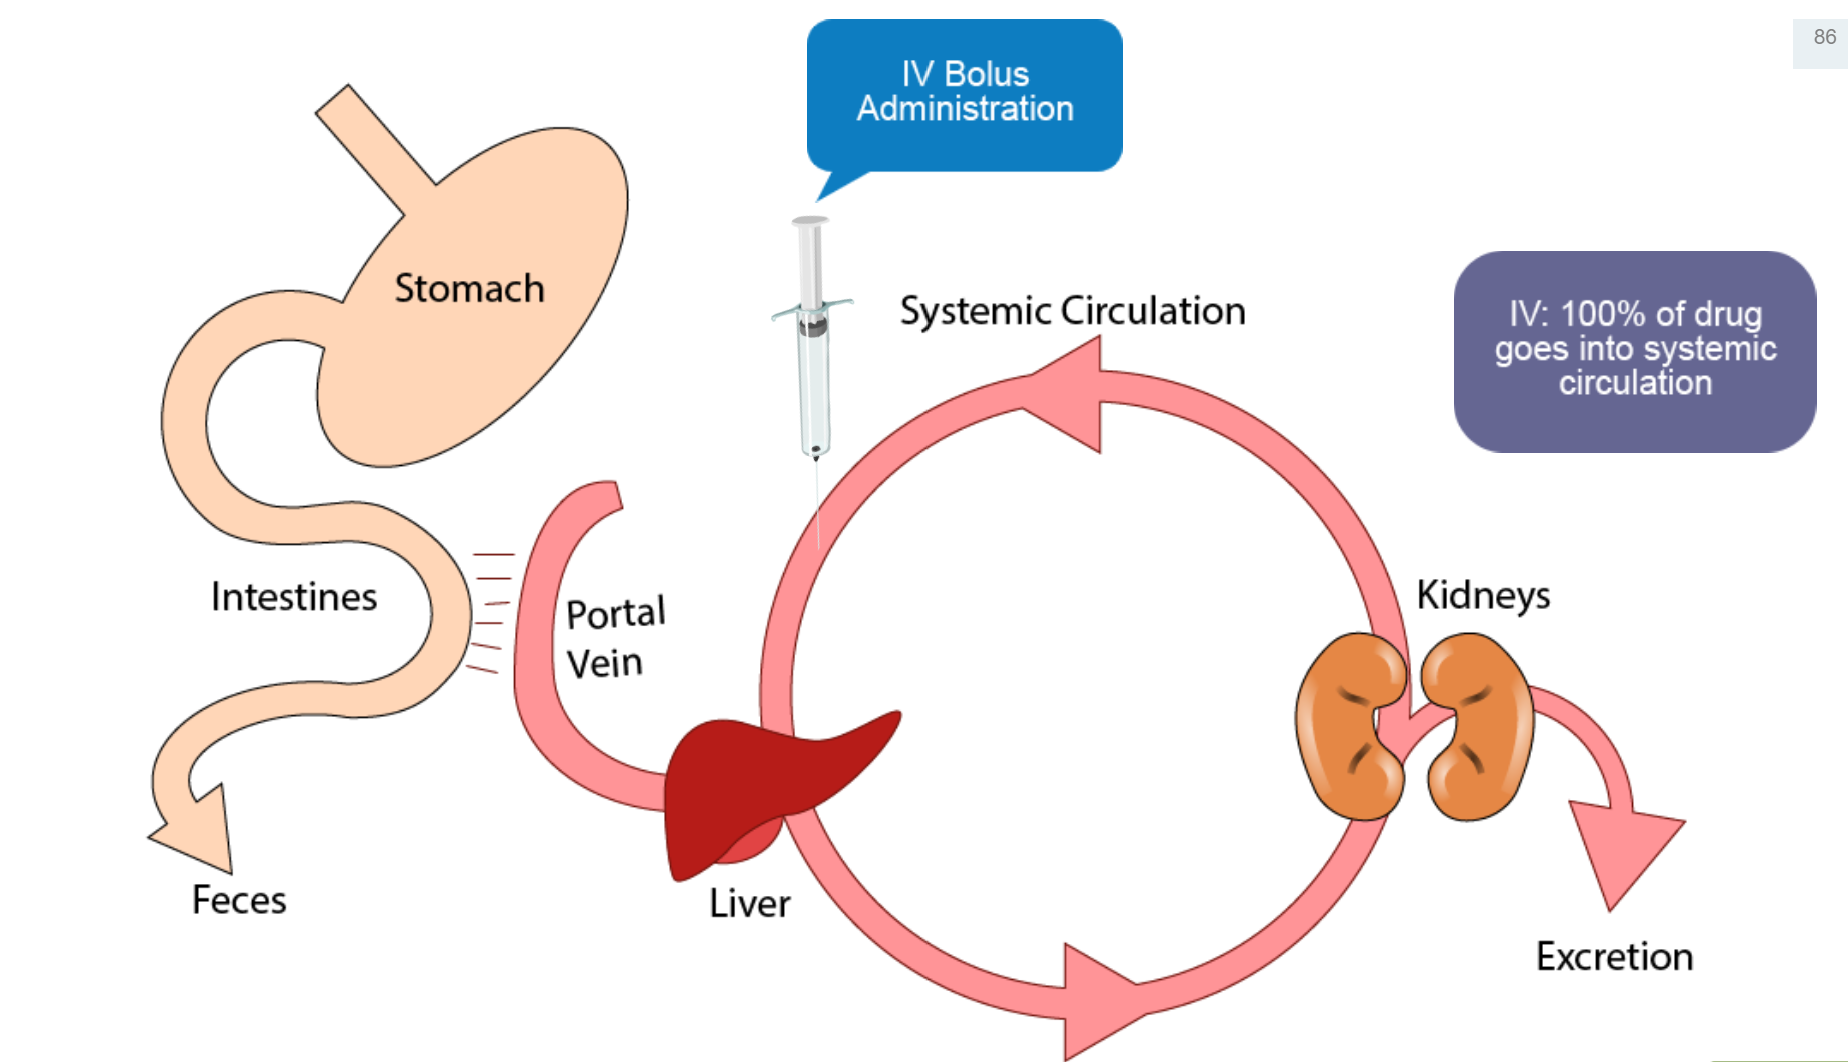
\includegraphics{./images/image-284829586.png}

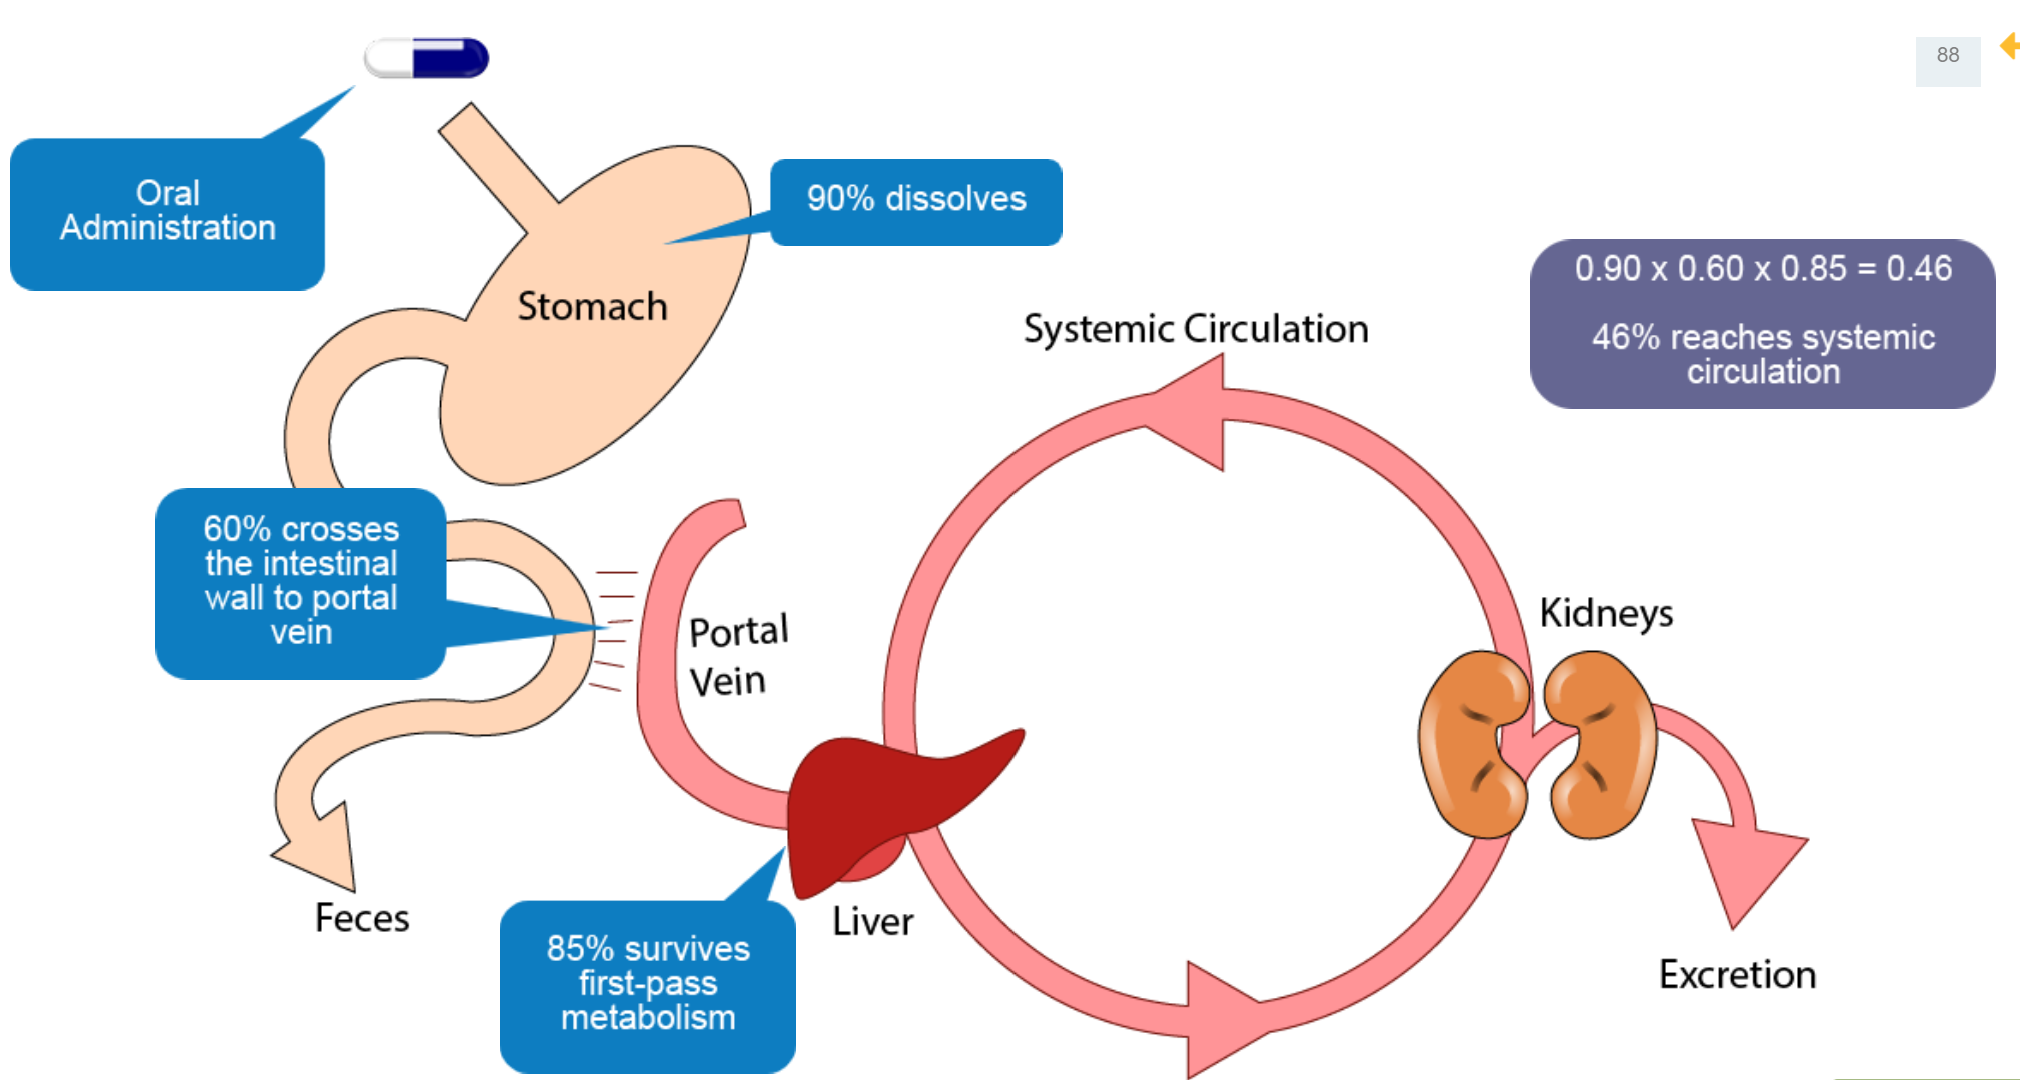
\includegraphics{./images/image-510239295.png}

\begin{itemize}
\tightlist
\item
  it is difficult to obtain all the ratios, so the overall ratio is
  called Bioavailability.
\end{itemize}

Bioavailability

\[
F = \frac{AUC_{oral}/Dose_{oral}}{AUC_{IV}/Dose_{IV}}
\]

\begin{itemize}
\item
  Intravenous: NCA parameters are V and Cl (F = 1)
\item
  Extravascular: NCA parameters are V/F and Cl/F (F\textless1)
\item
  Elimination = Metabolism (liver) + Excretion (Kidney)
\item
  Cl\textsubscript{total} = Cl\textsubscript{hepatic} +
  Cl\textsubscript{renal} + Cl\textsubscript{other}
\item
  Cl\textsubscript{renal} = A\textsubscript{e} (amount of drug excreted
  in the urine)/ AUC\textsubscript{plasma}
\item
  Calculation of Clearance from NCA:
\end{itemize}

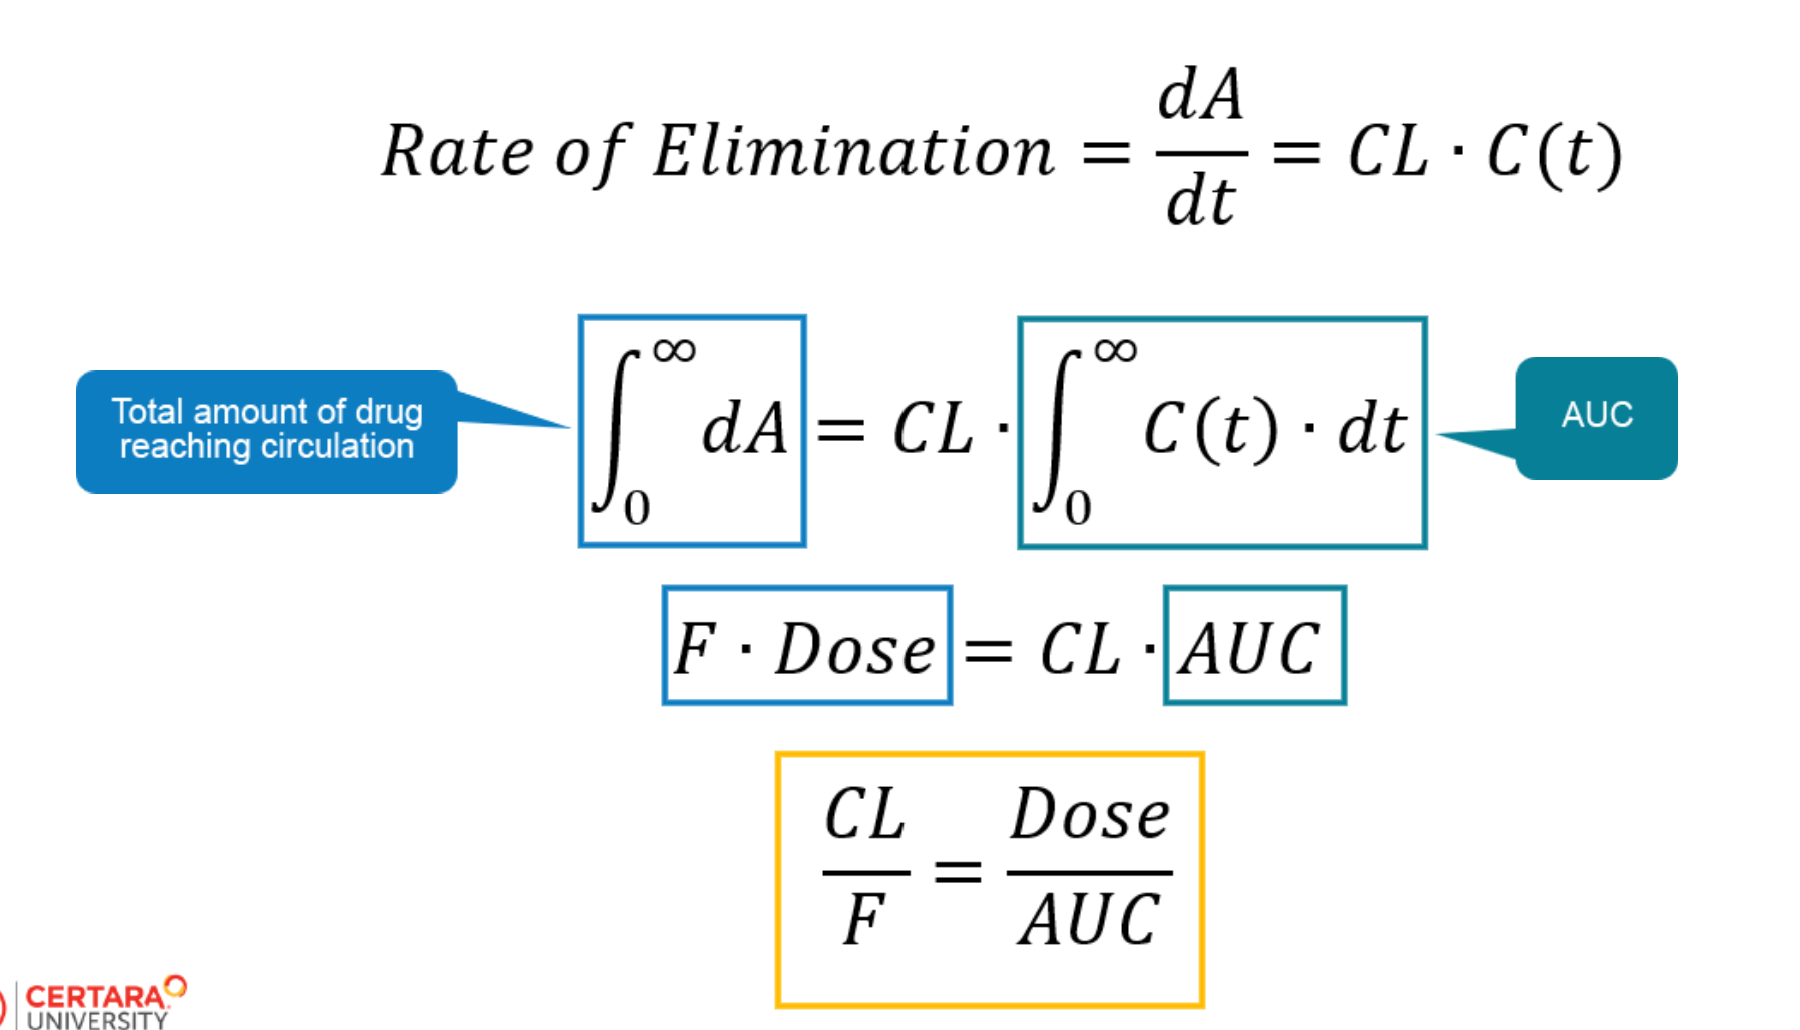
\includegraphics{./images/image-281401148.png}

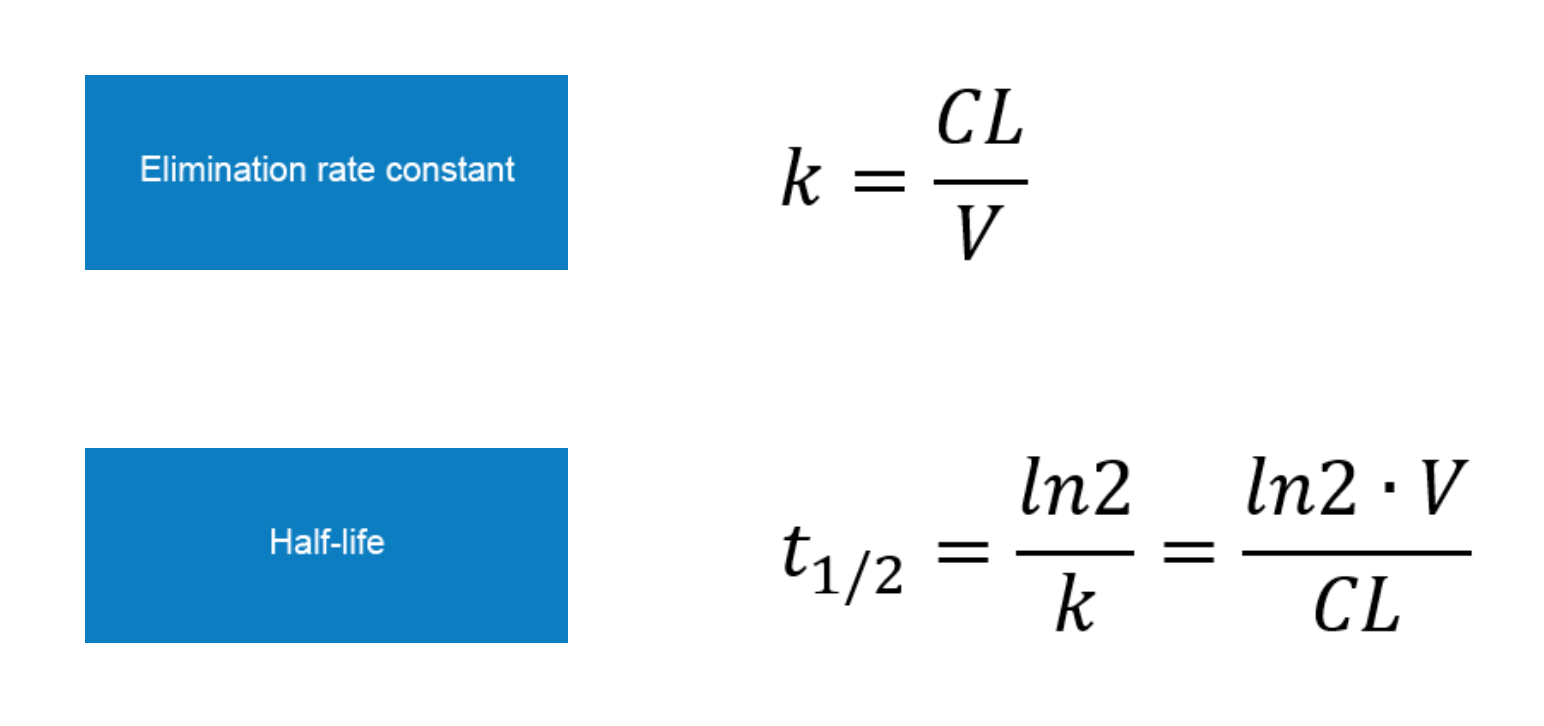
\includegraphics{./images/image-2093126627.png}

You get the following from NCA

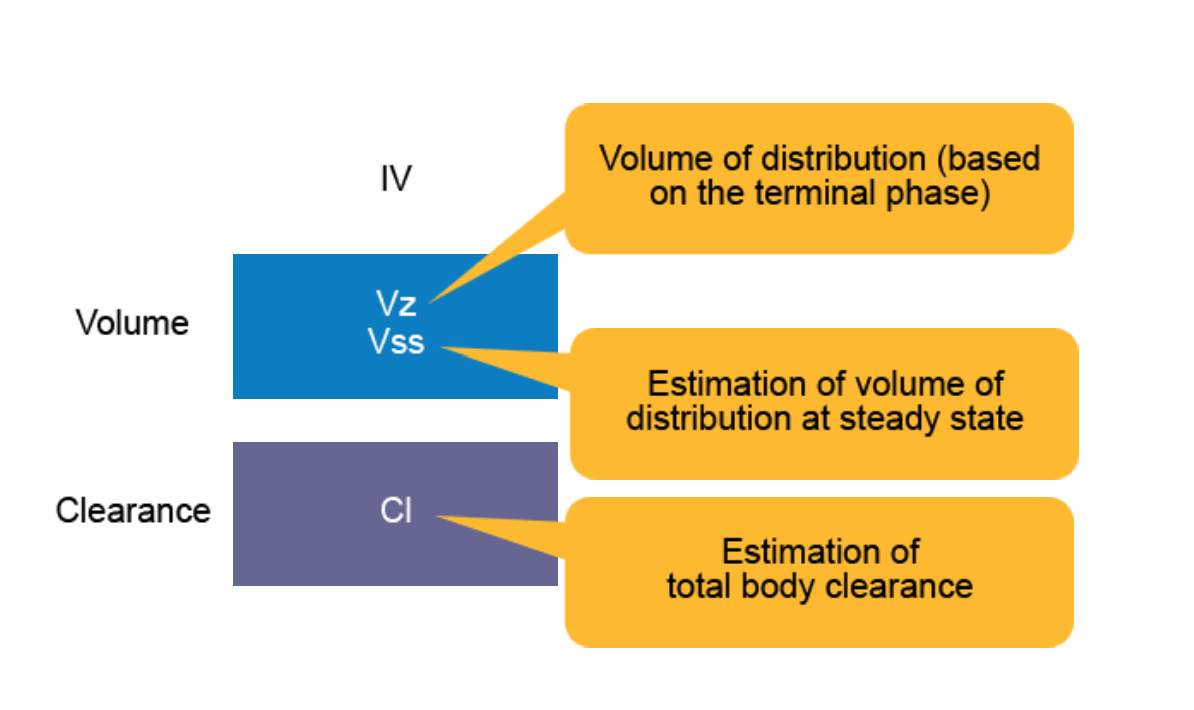
\includegraphics{./images/image-438969836.png}

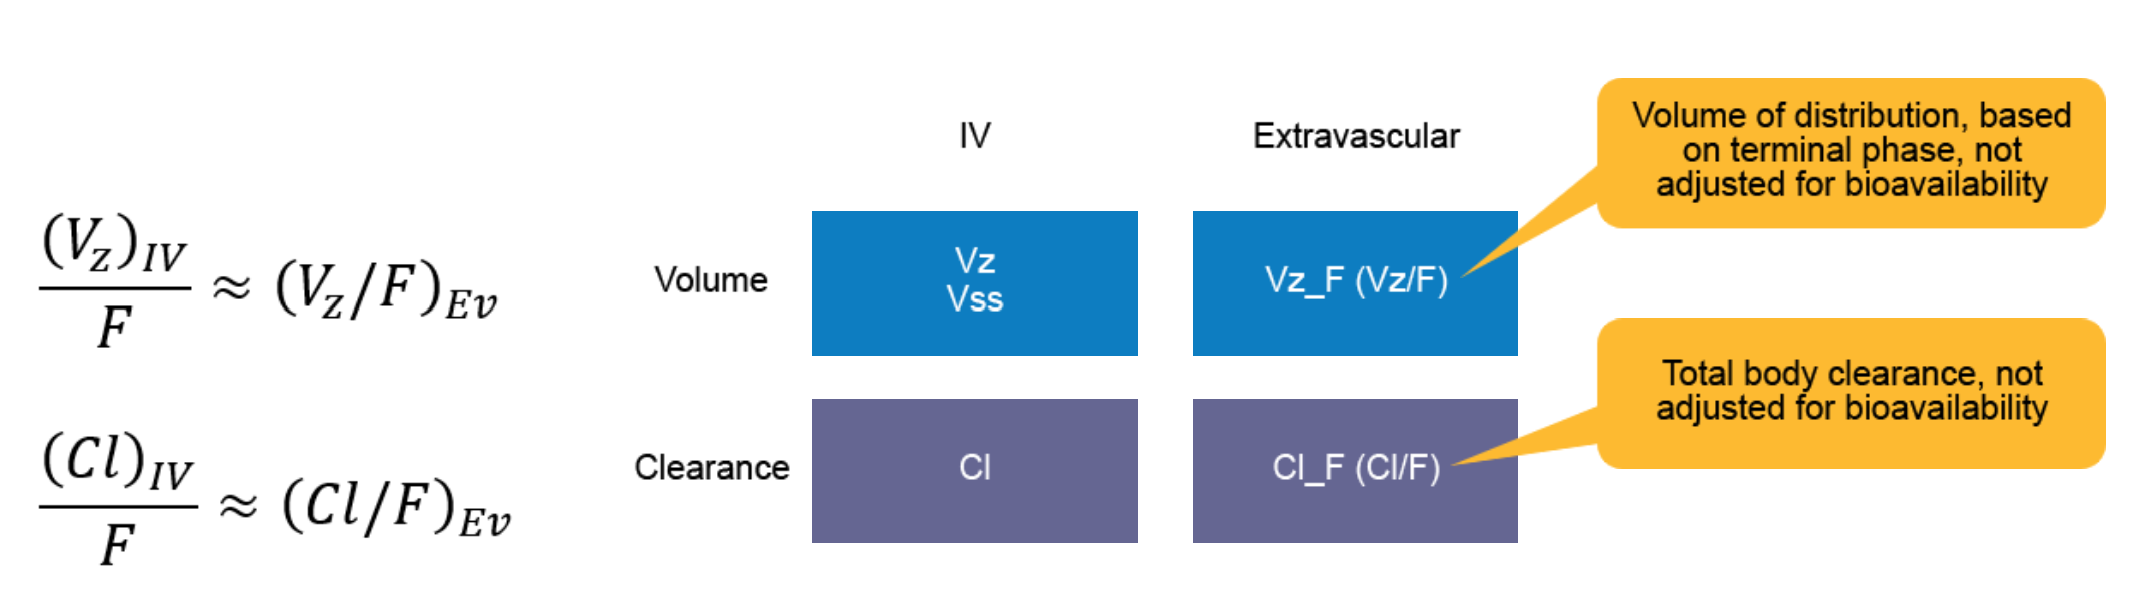
\includegraphics{./images/image-1032710582.png}

\hypertarget{linear-vs-log}{%
\subsection{Linear vs Log}\label{linear-vs-log}}

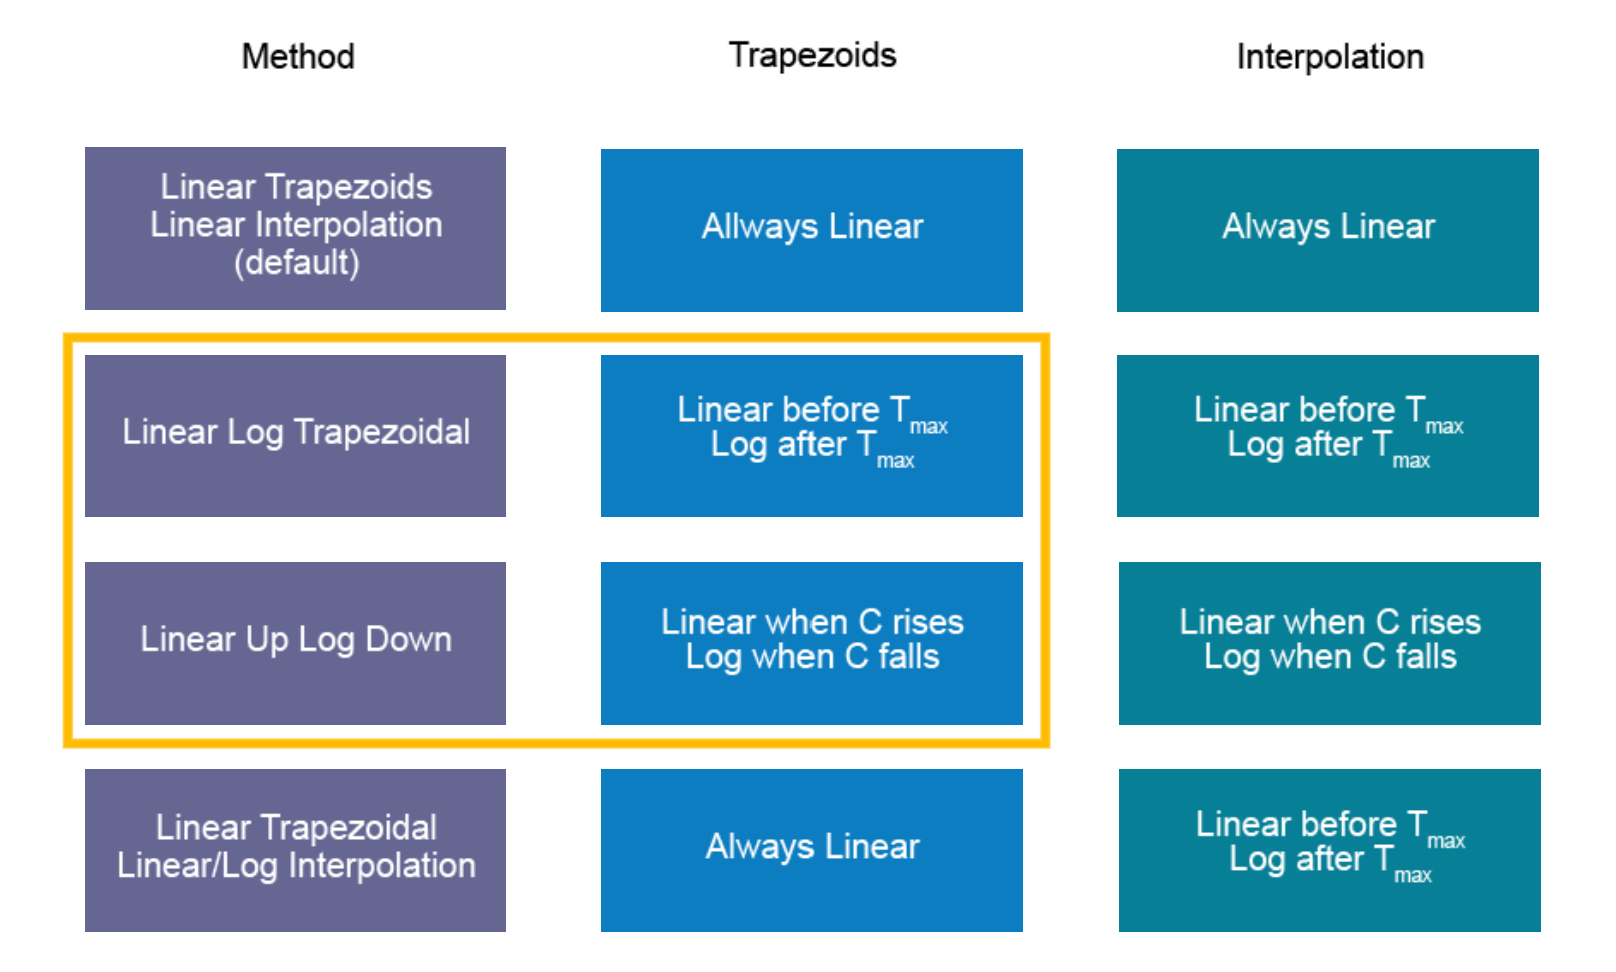
\includegraphics{./images/image-1313806547.png}

\bookmarksetup{startatroot}

\hypertarget{winnonlin-modeling123-od}{%
\chapter{WinNonlin Modeling(123-OD)}\label{winnonlin-modeling123-od}}

See Alam (2006) for additional discussion on modeling

\hypertarget{what-is-a-model}{%
\section{What is a Model}\label{what-is-a-model}}

\begin{itemize}
\tightlist
\item
  a mathematical abstraction
\item
  below is a diagram of a typical PK model
\end{itemize}

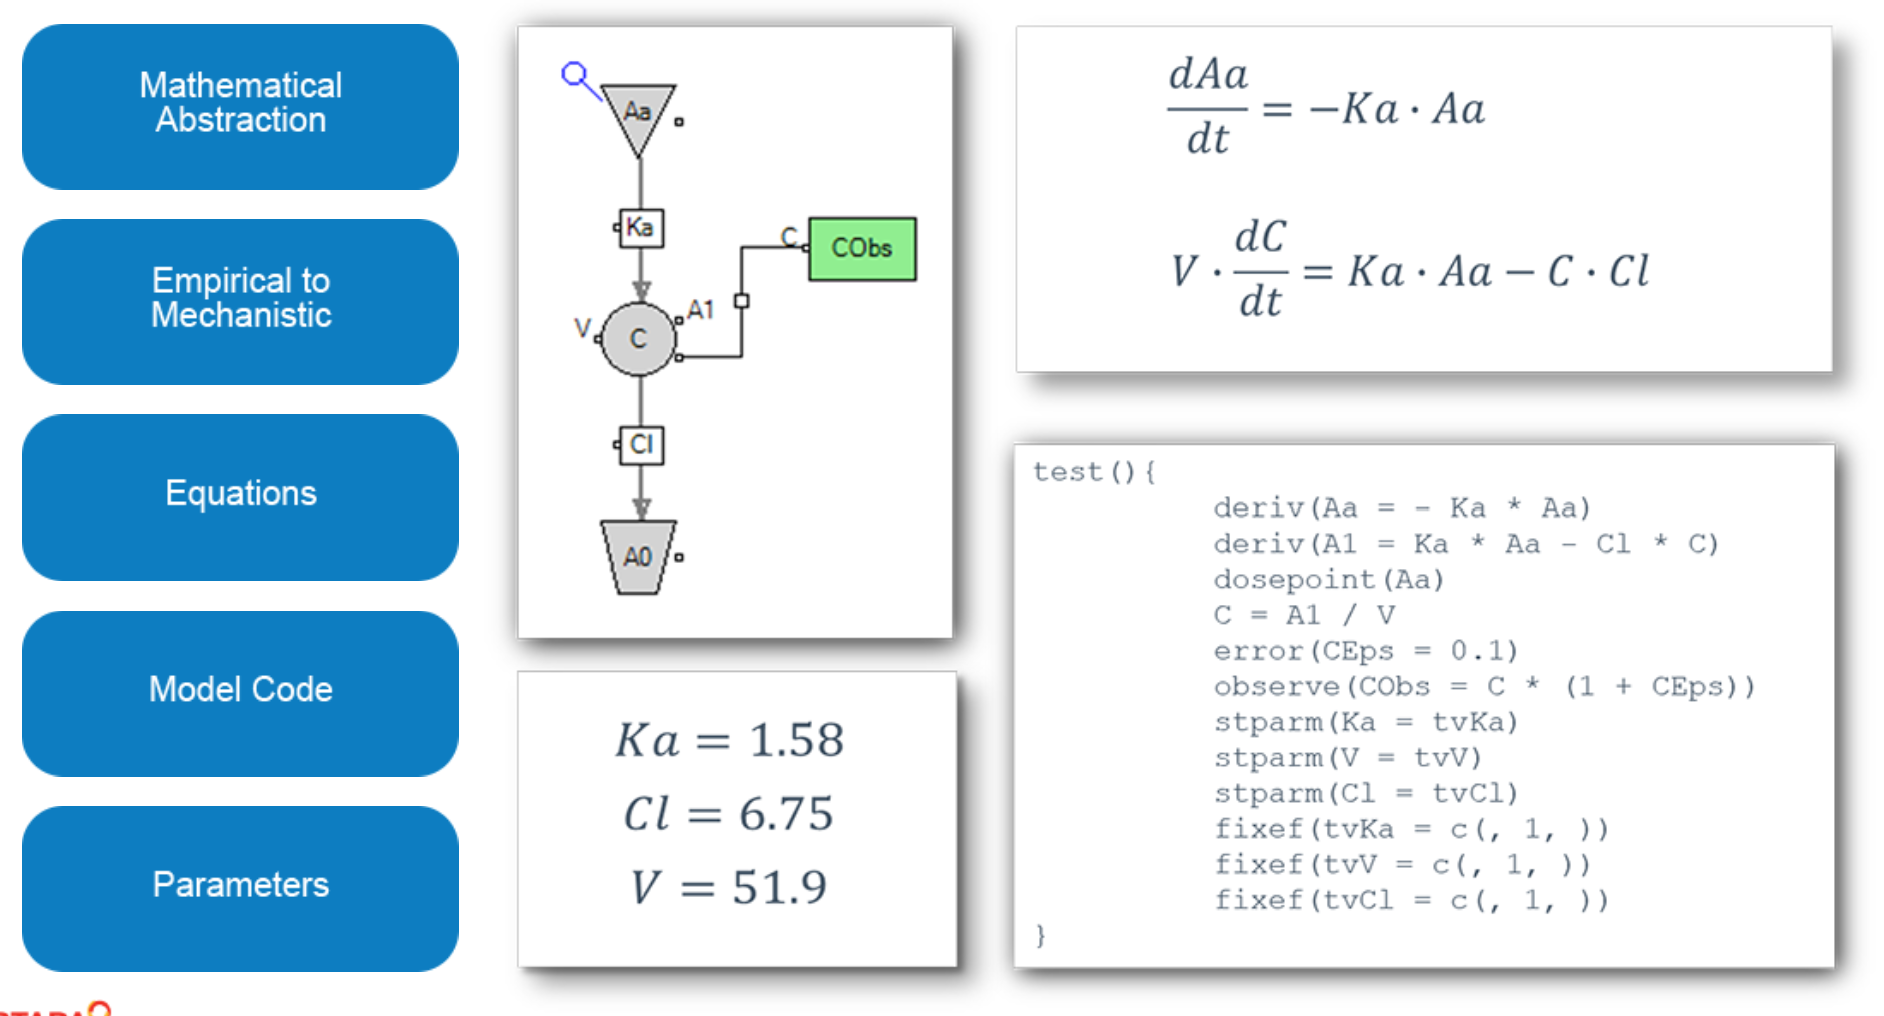
\includegraphics{./img/model-1.png}- The movement of drug through the
body is usually much more complicated than depicted in the diagram but
even a simple model such as this can mimic the shape of the observed
data and allow us to make predictions.

\begin{itemize}
\tightlist
\item
  models can be anywhere from purely empirical to purely mechanistic\\
\item
  empirical model is used just because it fits the data without drawing
  too many conclusions about the process that the drug undergoes while
  being absorbed distributed metabolized and eliminated
\item
  a mechanistic model accounts for many of the processes that the drug
  is known to undergo
\item
  the model in the diagram is translated into a series of differential
  equations\\
\item
  The equations that describe the model are converted into model code in
  Phoenix
\item
  Parameter values
\end{itemize}

\hypertarget{parameterization}{%
\section{Parameterization}\label{parameterization}}

\begin{itemize}
\tightlist
\item
  parameterization refers to the type of parameters that are used in the
  model
\item
  examples include clearance parameters, micro parameters and macro
  parameters
\end{itemize}

let's see how these differ first let's consider

clearance parameters

\begin{itemize}
\tightlist
\item
  the most widely used
\item
  The parameters in this model are the absorption rate constant, the
  clearance and the volume
\item
  we suggest using clearance parameters when possible because

  \begin{itemize}
  \tightlist
  \item
    clearances are physiologically relevant and
  \item
    clearance-based models tend to be more stable
  \item
    it is also easy to obtain initial estimates by using parameters from
    NCA
  \end{itemize}
\end{itemize}

micro-parameters

\begin{itemize}
\tightlist
\item
  All the transport is defined in terms of rate constants
\item
  These models are also widely used particularly for more mechanistic
\item
  In the picture model both KA and Ke are rate constants and v is the
  volume
\end{itemize}

macro parameter

\begin{itemize}
\tightlist
\item
  These were the first type of parameters to be used in PK modeling
\item
  PK curve is given by an equation that is combination of one or more
  exponentials
\item
  these parameters are not directly related to the phyiology
\end{itemize}

Clearance paremeters and microparameters are easily convertable. Let's
look at the

Firts, let's consider microparameters:

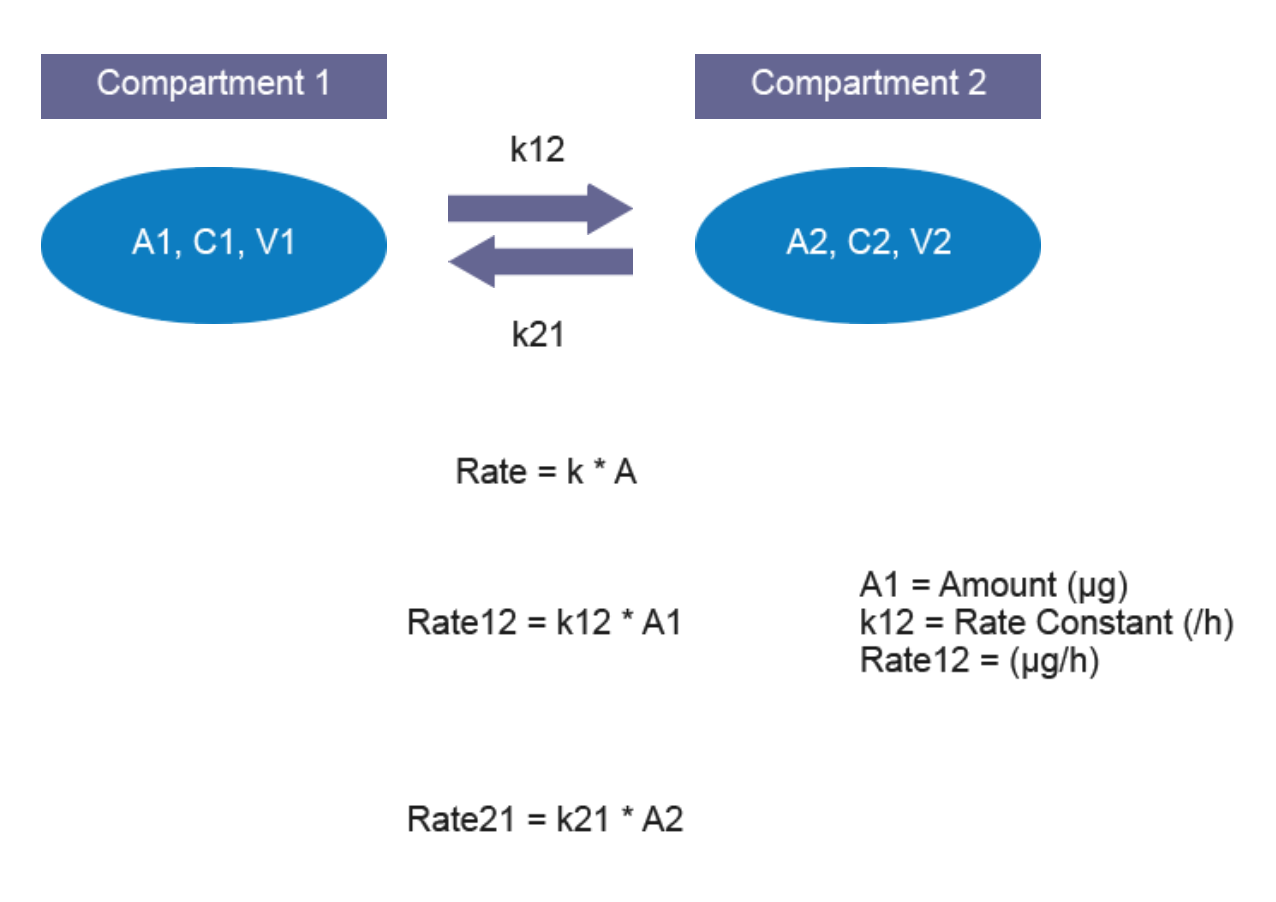
\includegraphics[width=5.96875in,height=\textheight]{./img/param-2.png}

- drug can move in both direction k: rate constants A ;amount of drug in
the originative compartment

Next the clearance parameters
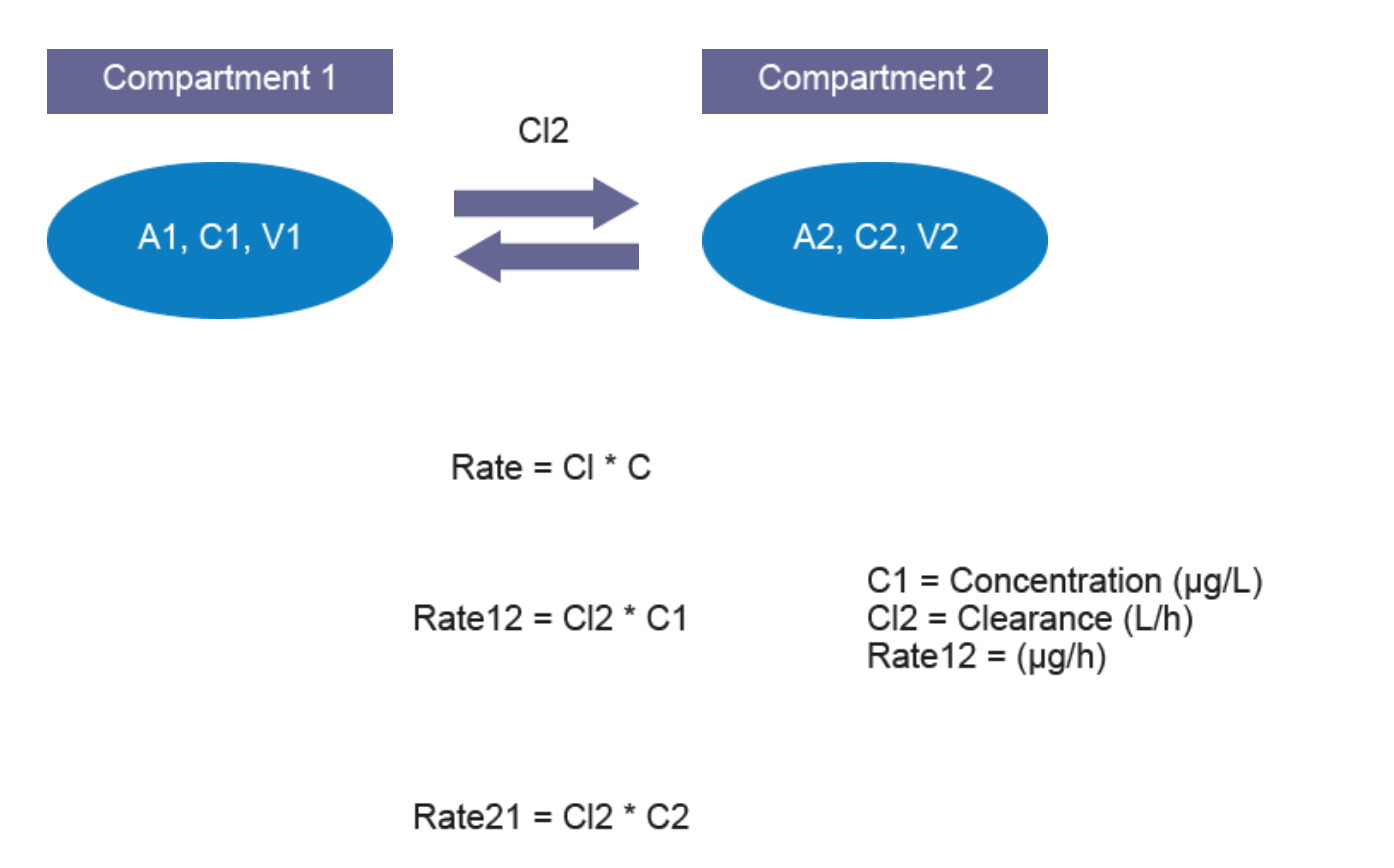
\includegraphics[width=5.94792in,height=\textheight]{./img/param-3.png}

Clearance and microcompartment models are usually equivalent and gives
similar results. However, clearance models are more commonly used.

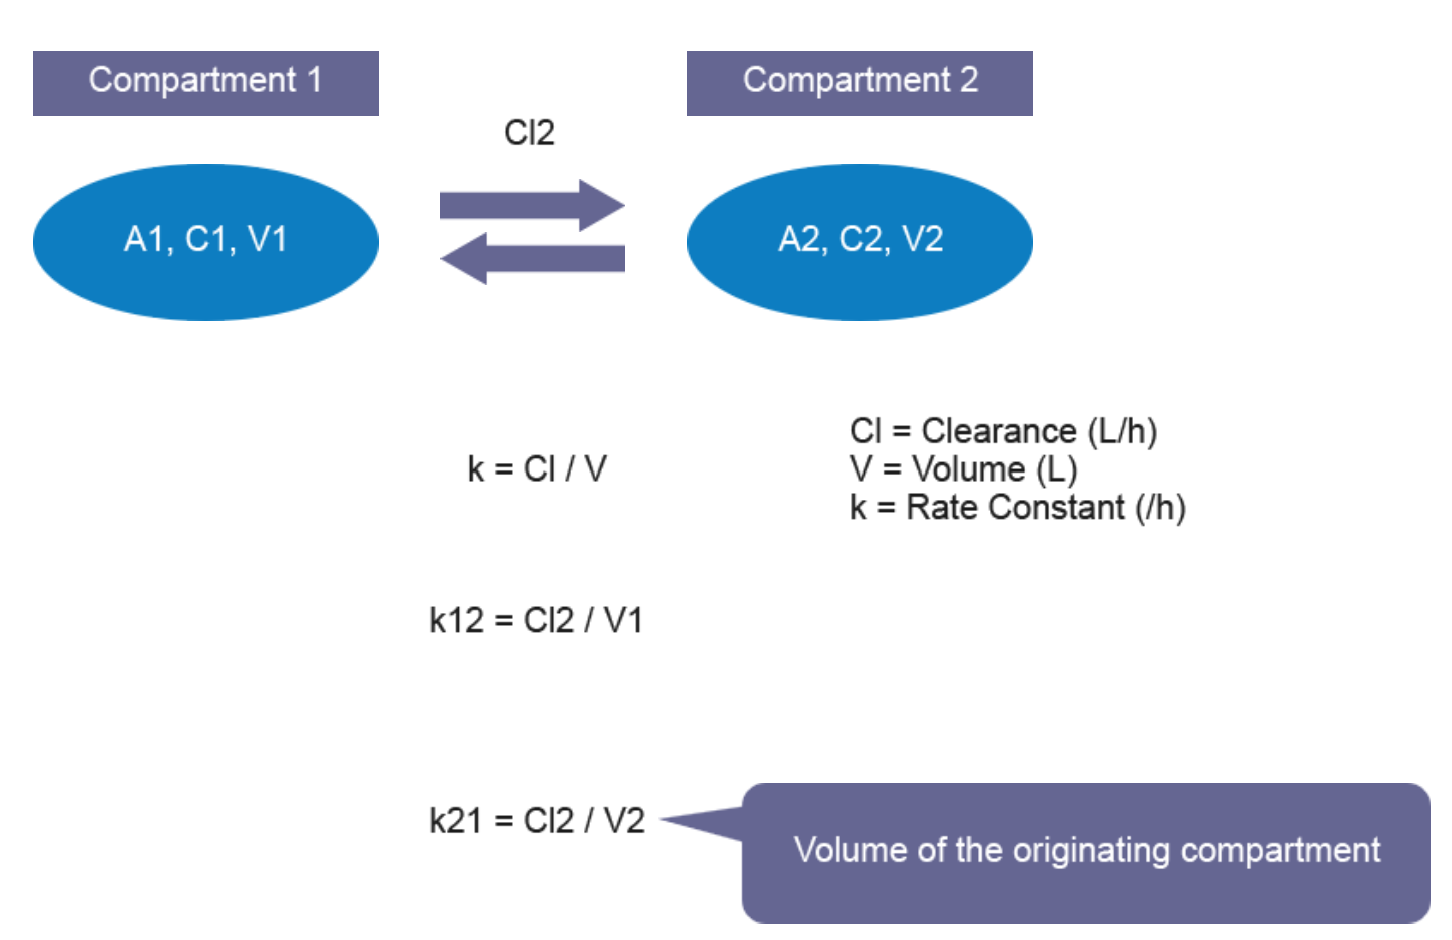
\includegraphics{./img/param-4.png}

\hypertarget{administration}{%
\subsection{administration}\label{administration}}

the way the drug is administered has a large effect on the shape of the
PK curve. three types of administration

\begin{enumerate}
\def\labelenumi{\arabic{enumi}.}
\tightlist
\item
  Extravascular
\end{enumerate}

\begin{itemize}
\tightlist
\item
  Oral, subcautaneous, intervanious, etc any kind of administration that
  involves an absorption
\item
  there is a depot compartment that receives the dose
\item
  in Phoenix the dose point is indicated with the blue syringe, The name
  of the absorption compartment is AA and the absorption rate constant
  is KA any administration
\end{itemize}

\begin{enumerate}
\def\labelenumi{\arabic{enumi}.}
\setcounter{enumi}{1}
\tightlist
\item
  Intravenous (IV infusion or IV bolus)
\end{enumerate}

\begin{itemize}
\tightlist
\item
  Delivered at a constant rate for a defined duration or rate
\item
  there is no absorption process and the dose point delivers the drug
  directly into the central compartment
\end{itemize}

let's compare the shapes of PK curves resulting from different
administration methods here are three simulations all with - a dose of
5,000 micrograms - a volume of 100 liters - a clearance of 20 liters per
hour and - an absorption rate constant ka of 1 per hour

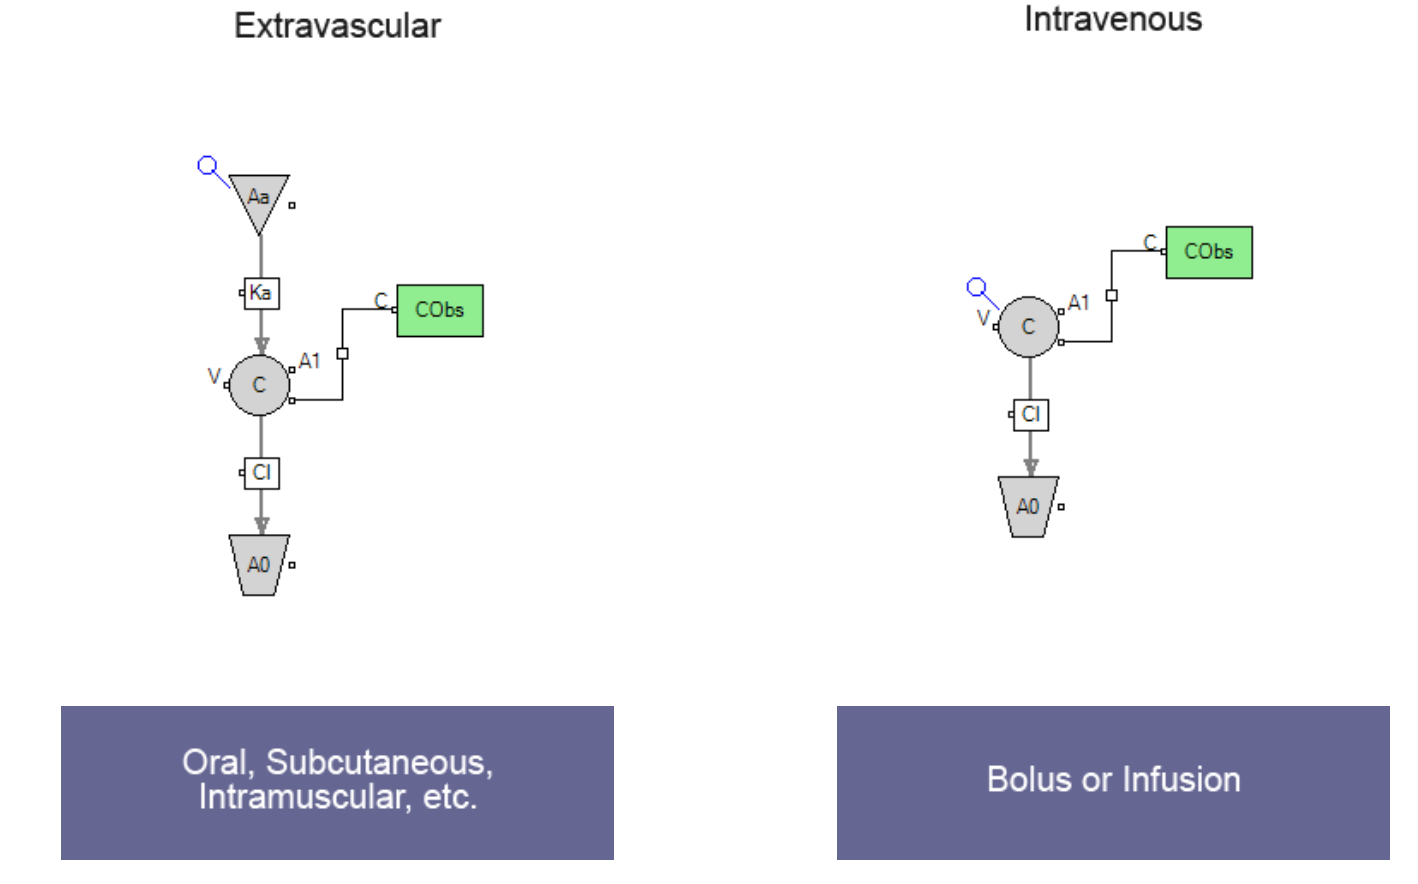
\includegraphics{./img/admin-1.png}

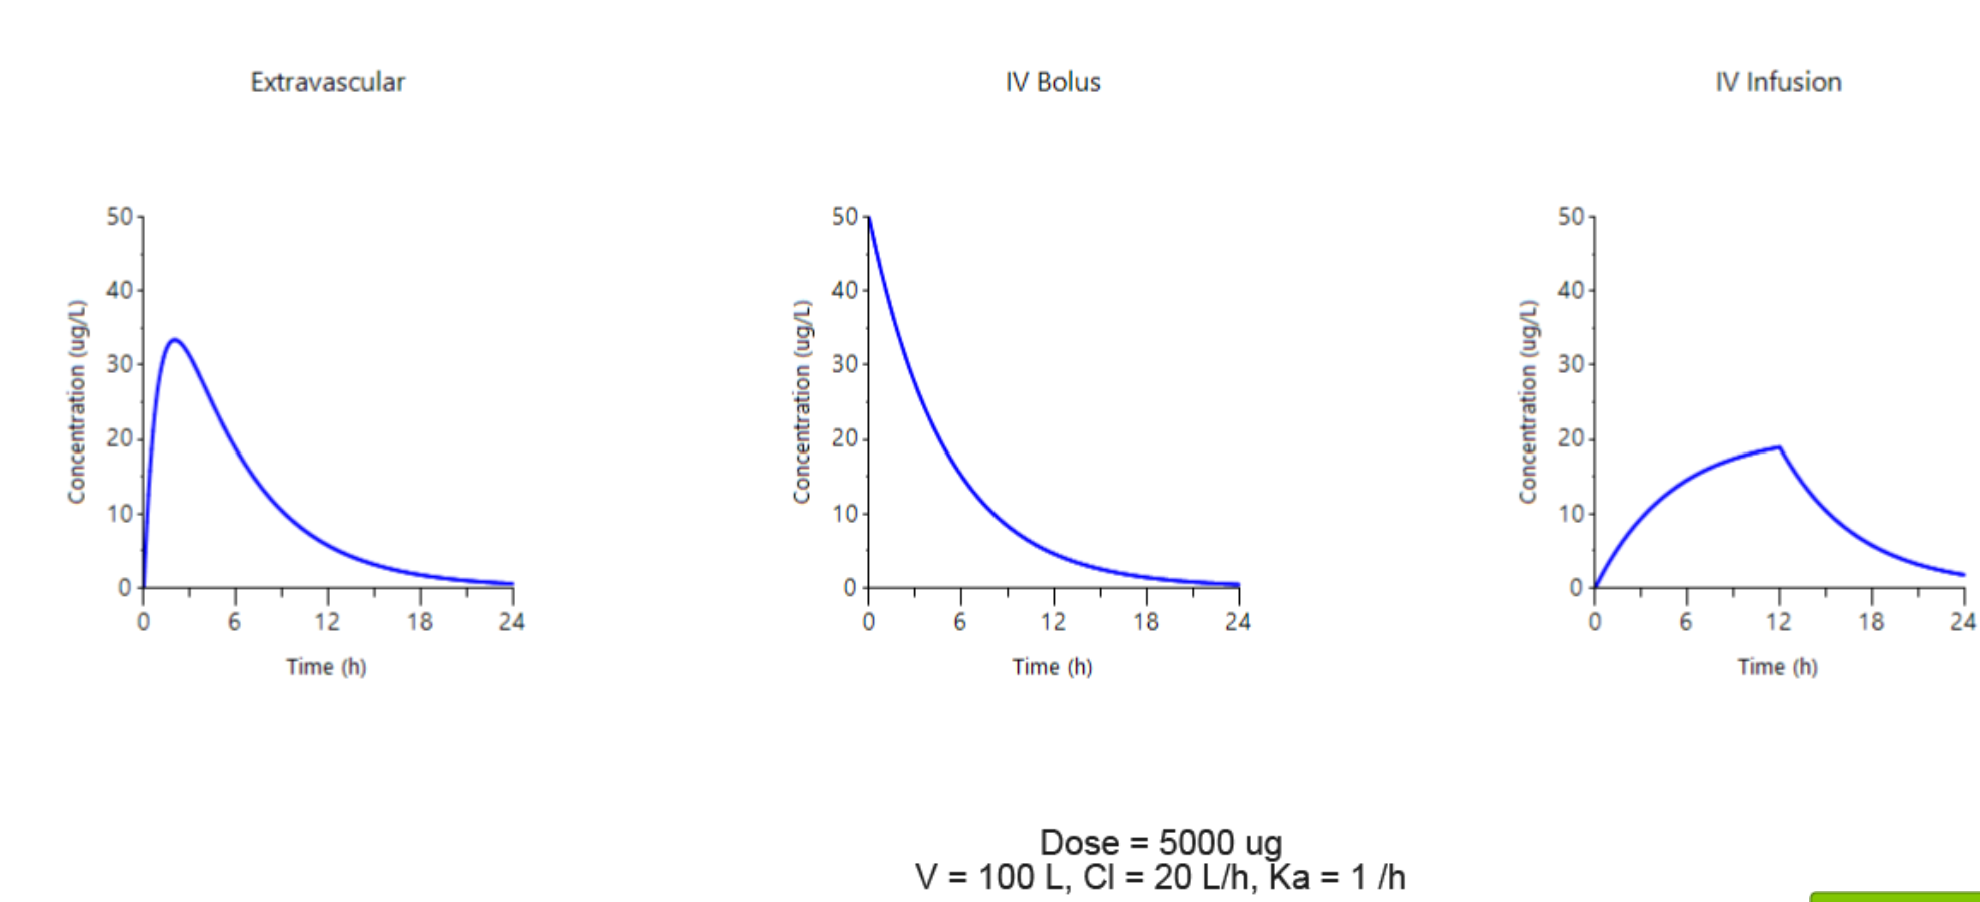
\includegraphics{./img/admin-2.png}

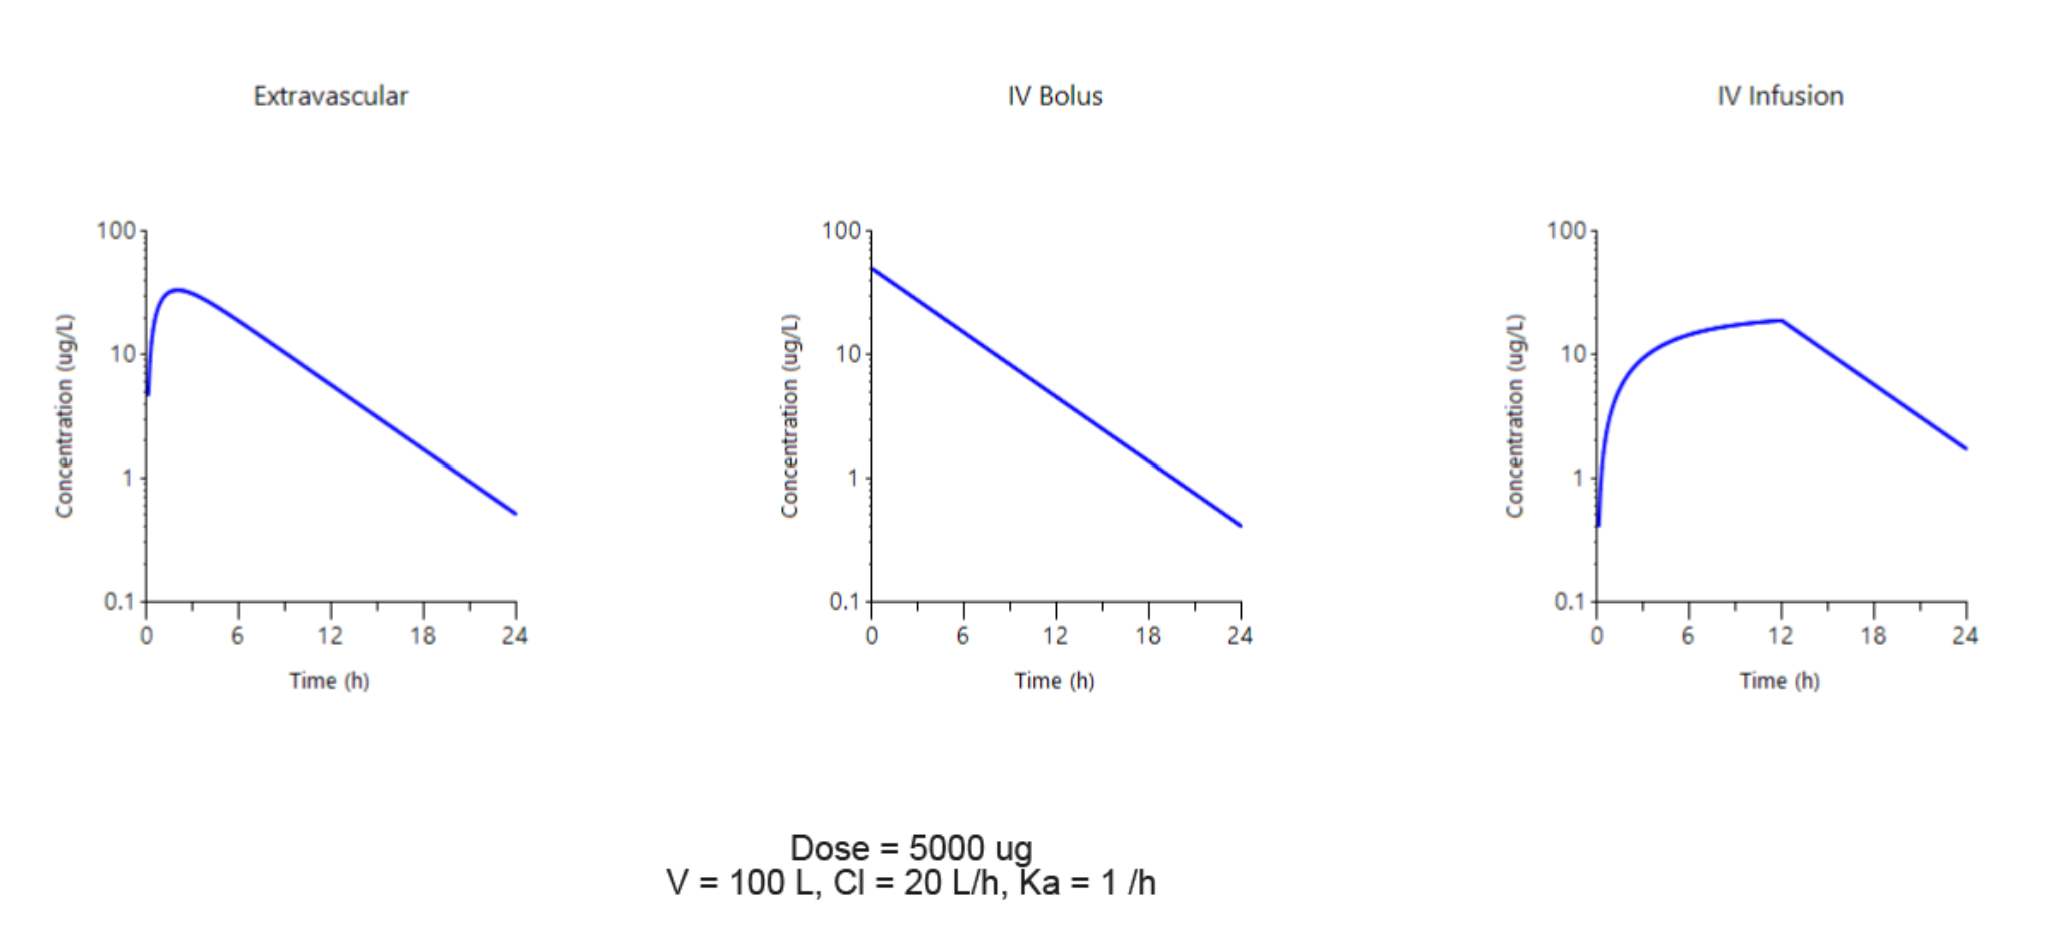
\includegraphics{./img/admin-3.png}

\begin{itemize}
\tightlist
\item
  the elimination phase is linear in all three plots and there is no
  distribution phase seen
\end{itemize}

\hypertarget{model-structure}{%
\section{4. model structure}\label{model-structure}}

\begin{itemize}
\tightlist
\item
  the model structure affects the shape of the pK profile
\item
  three different aspects of model structure

  \begin{itemize}
  \tightlist
  \item
    number of compartments
  \item
    presence or absence of a time lag
  \item
    saturating elimination
  \end{itemize}
\end{itemize}

The effect of the number of compartments:

one compartment model is the simplest

\begin{itemize}
\tightlist
\item
  one compartment extravascular model
\item
  has three parameters k a v and CL
\end{itemize}

Two comartment models adds a peripheral compartment which can take up
some of the drug - needed when there is a sizable distribution phase -
five parameters

three compartments - adds two more parameters V3 and CL3 - The three
compartment model is not used frequently
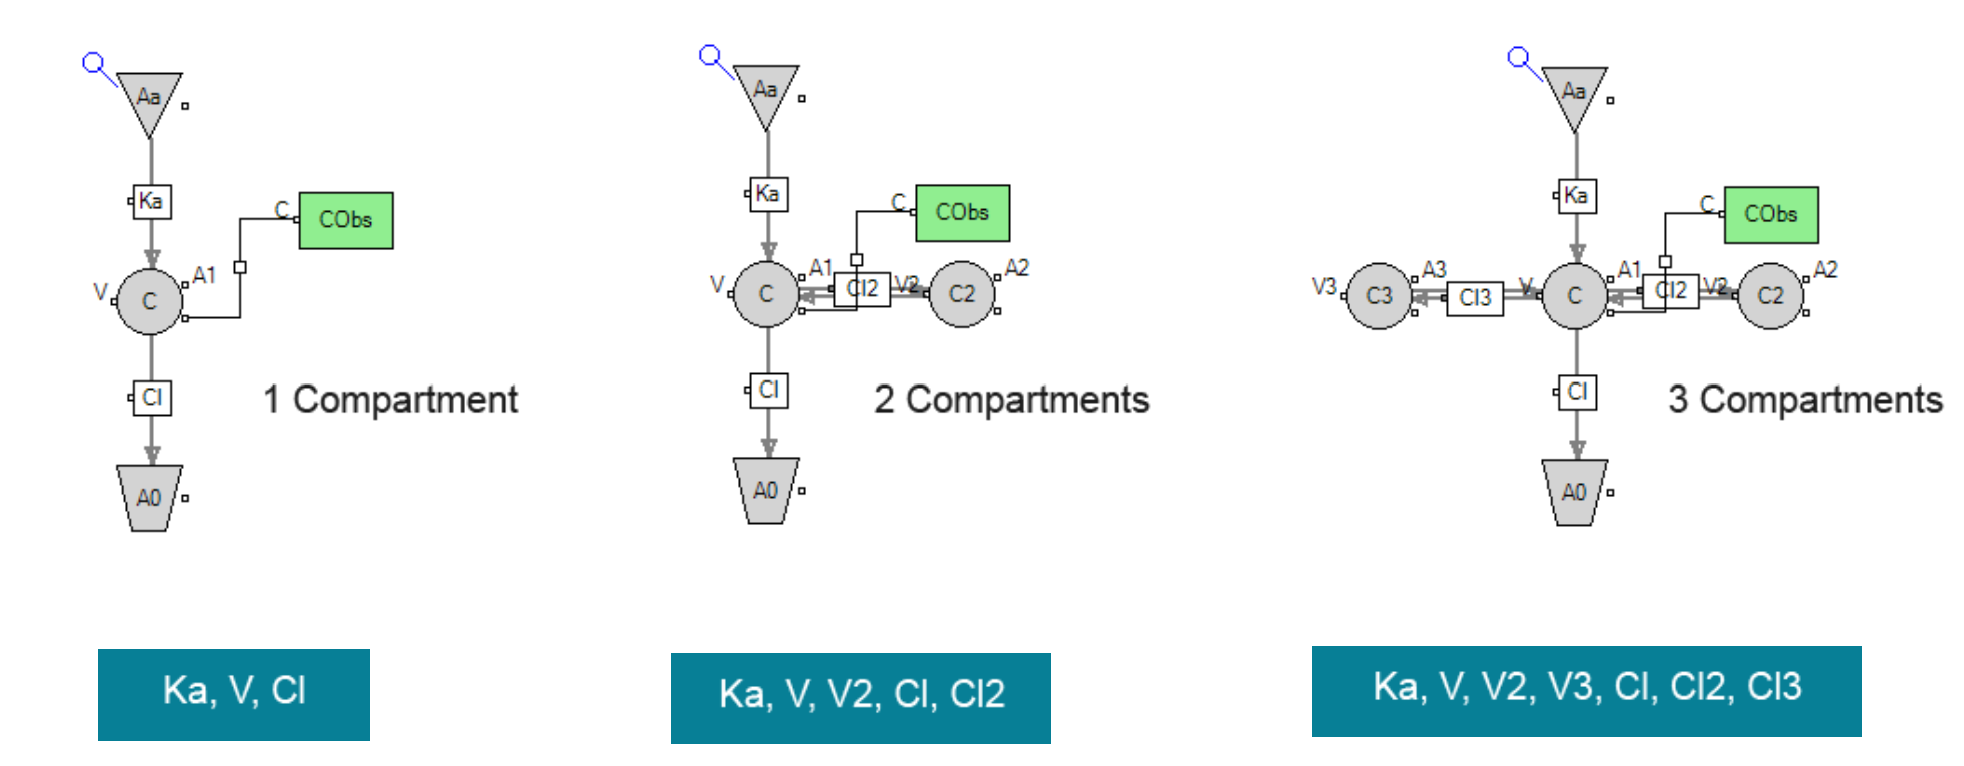
\includegraphics{./img/structure-1.png}

shape but the PK curve

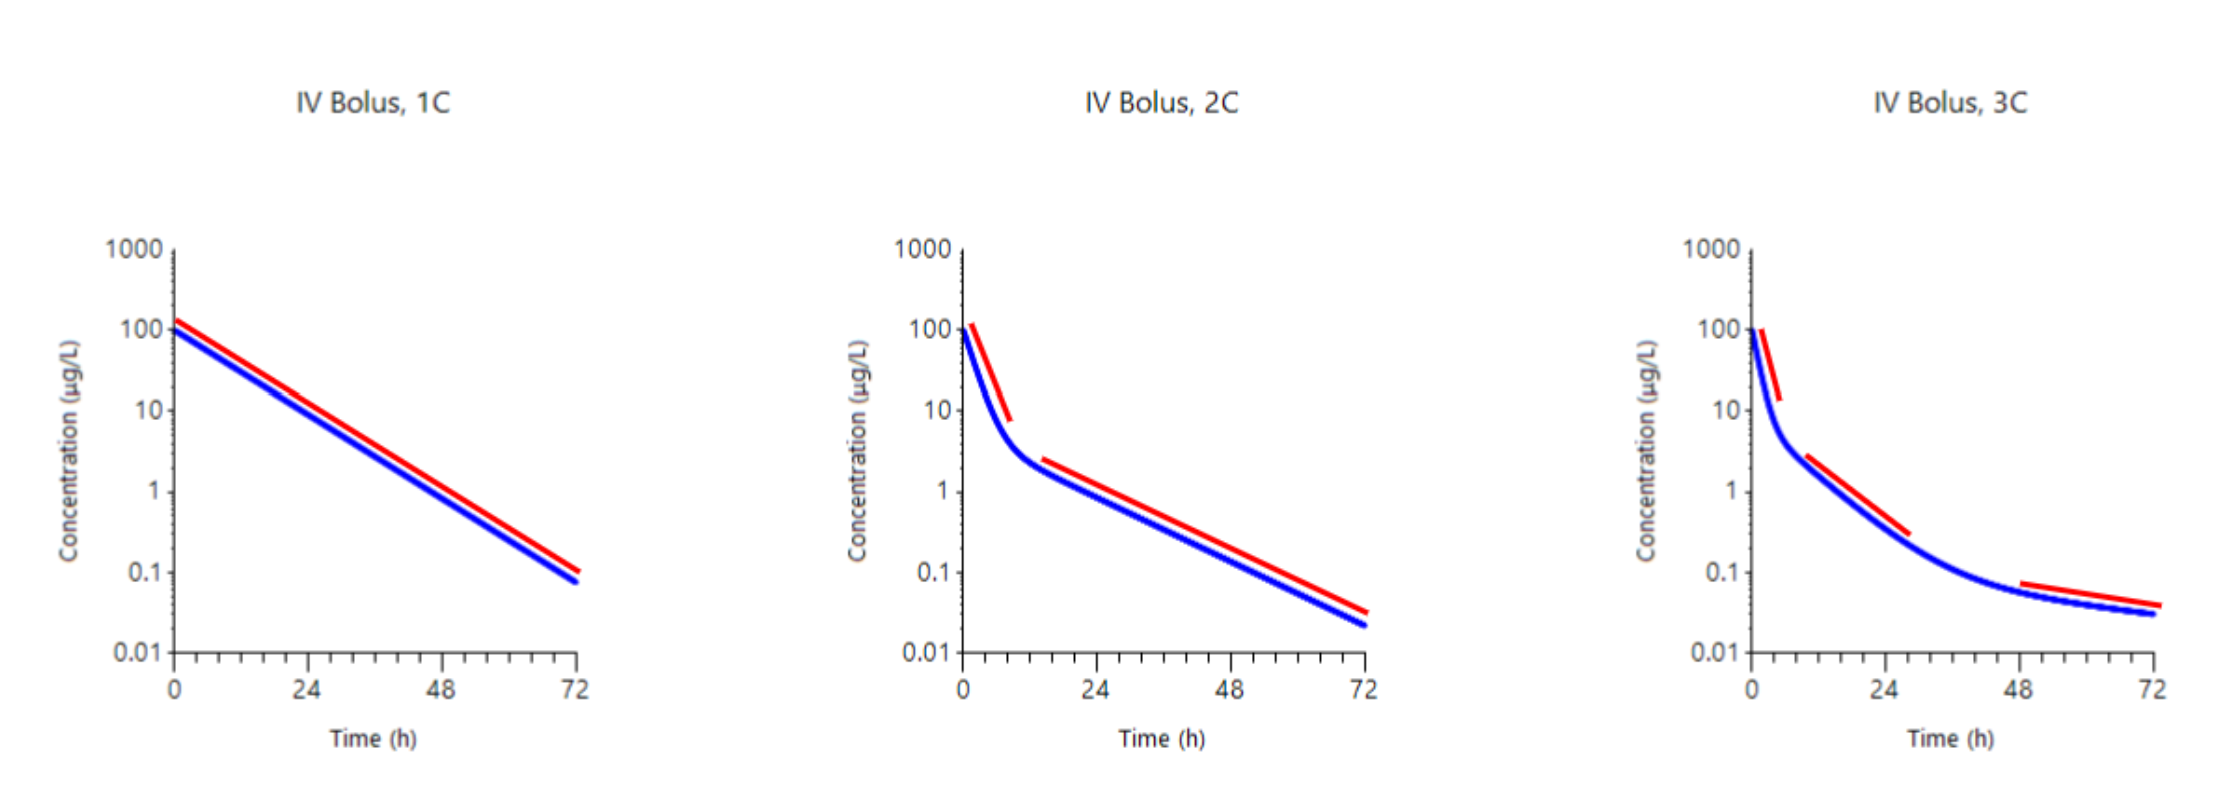
\includegraphics{./img/structure-2.png} - one compartment IV bolus model
is just a straight line when plotted on a log concentration axis - a two
compartment model is useful when there is a distribution phase that is
different than the elimination phase - The three compartment model can
have three distinct phases - it will not always be as apparent that
there are multiple phases instead of two distinct phases we may see a
general curvature that blends two or more phases together

corresponding extravascular Administration but

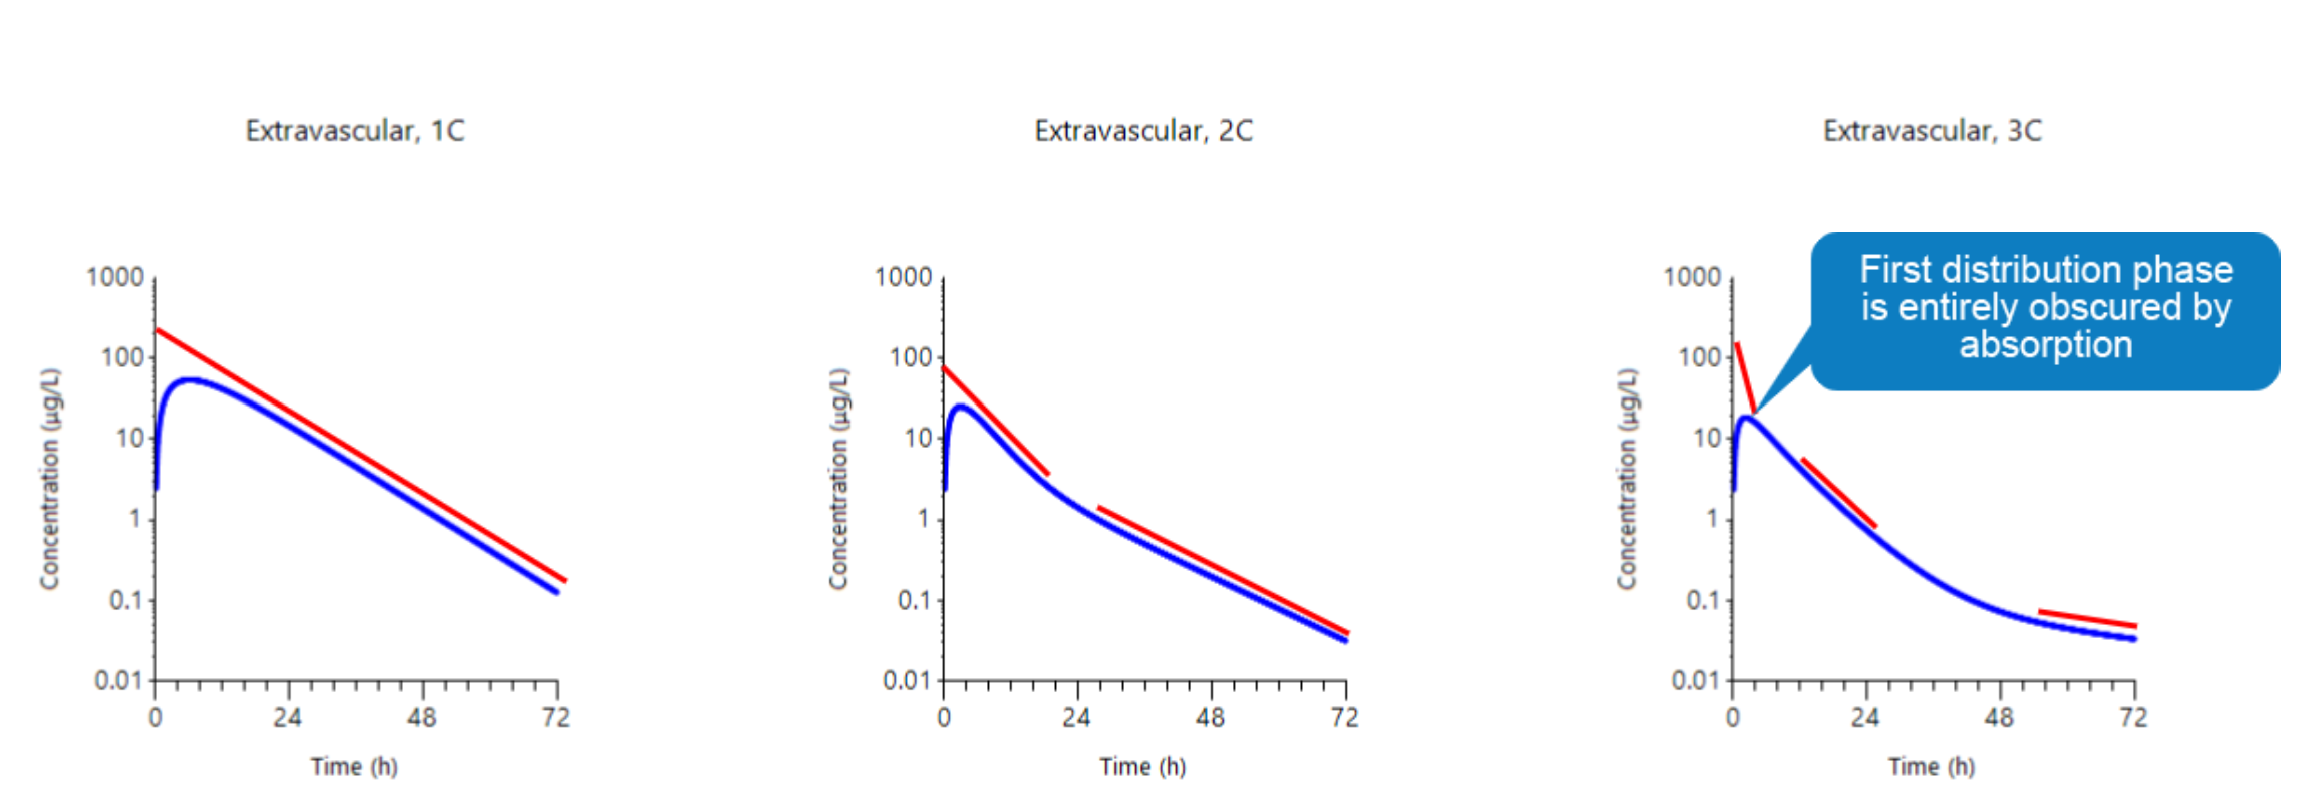
\includegraphics{./img/structure-3.png} - Early distribution phases can
become obscured because of the absorption phase - this is particularly
apparent in the three compartment model where the first distribution
phase is entirely obscured by the absorption

time lag

many drugs take some time to show up in systemic circulation and the
time lag is a way that we can account for this in our model

on the left is a model with the time lag and on the right is the
corresponding model without a time lag T-Lag is a parameter that causes
the absorption to be delayed Time lag has the same time units as the
time column

\begin{itemize}
\tightlist
\item
  add a time lag to your model if tmax does not fit properly
\item
  The model fit can then adjust both the KA and the T-Lag values to
  obtain and improve fit
\end{itemize}

saturation

\begin{itemize}
\item
  linear elimination saturation is often referred to as Michaela
\item
  replaces clearance parameter with Km and Vmax
  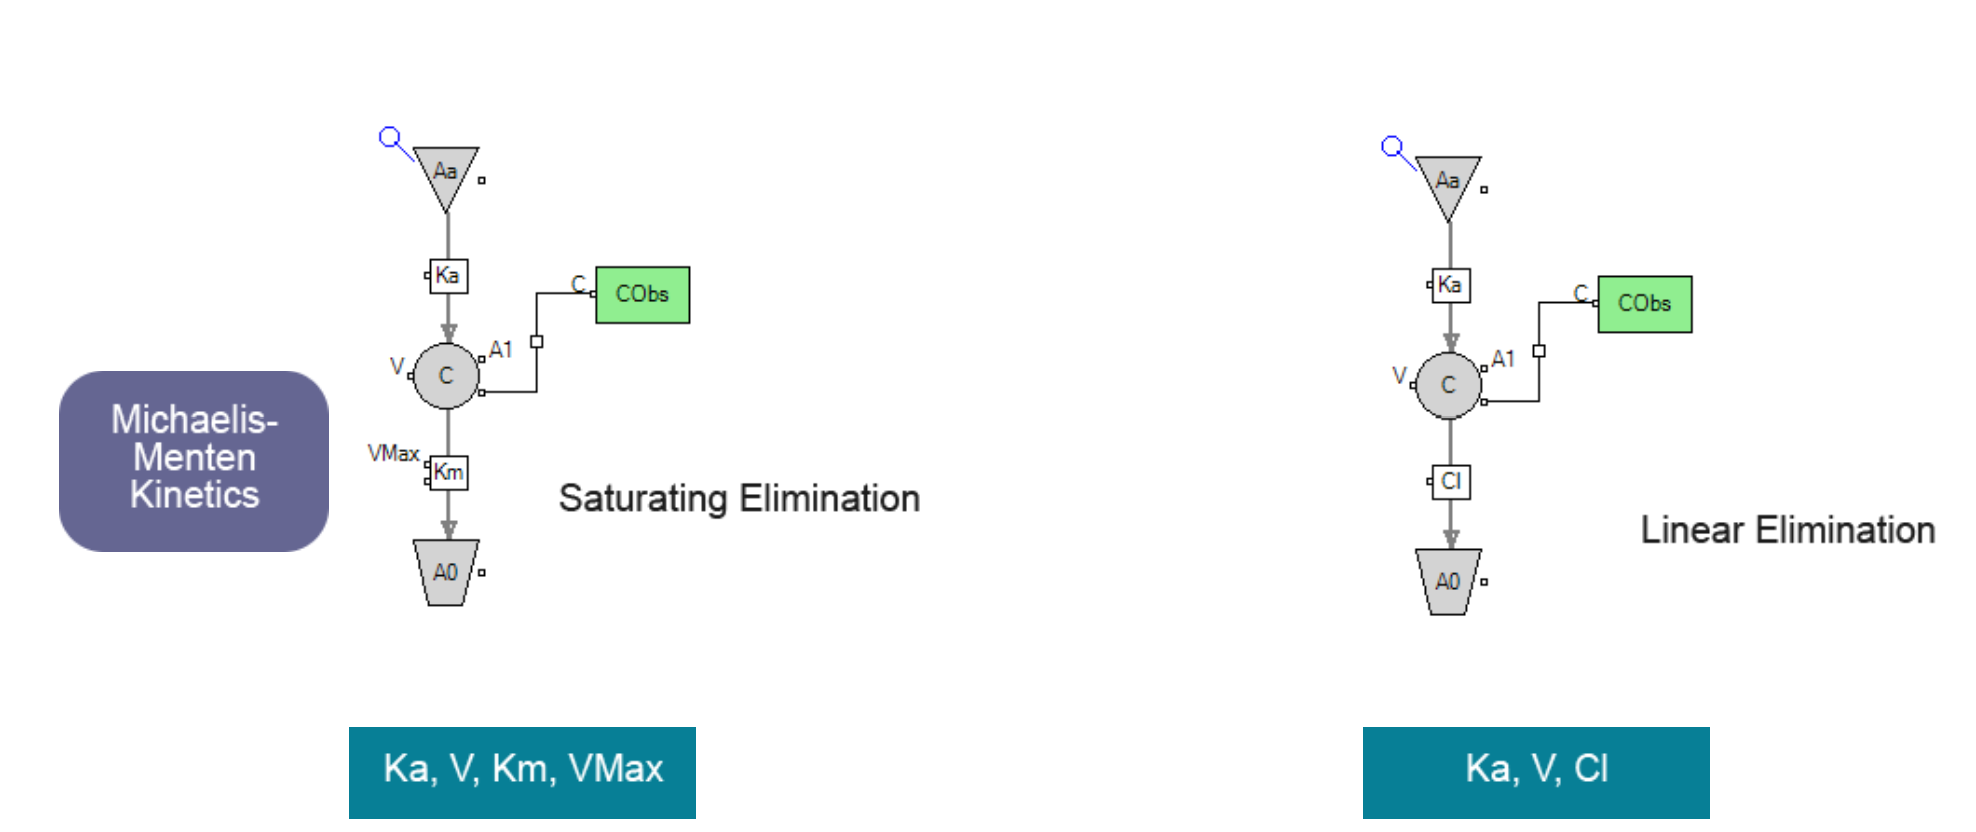
\includegraphics{./img/saturation-1.png} Clearance is no longer
  constant Clearance is depended on the concengtratino downward bend is
  characteristics of saturating kinetics saturation increased with
  higher doses
\item
  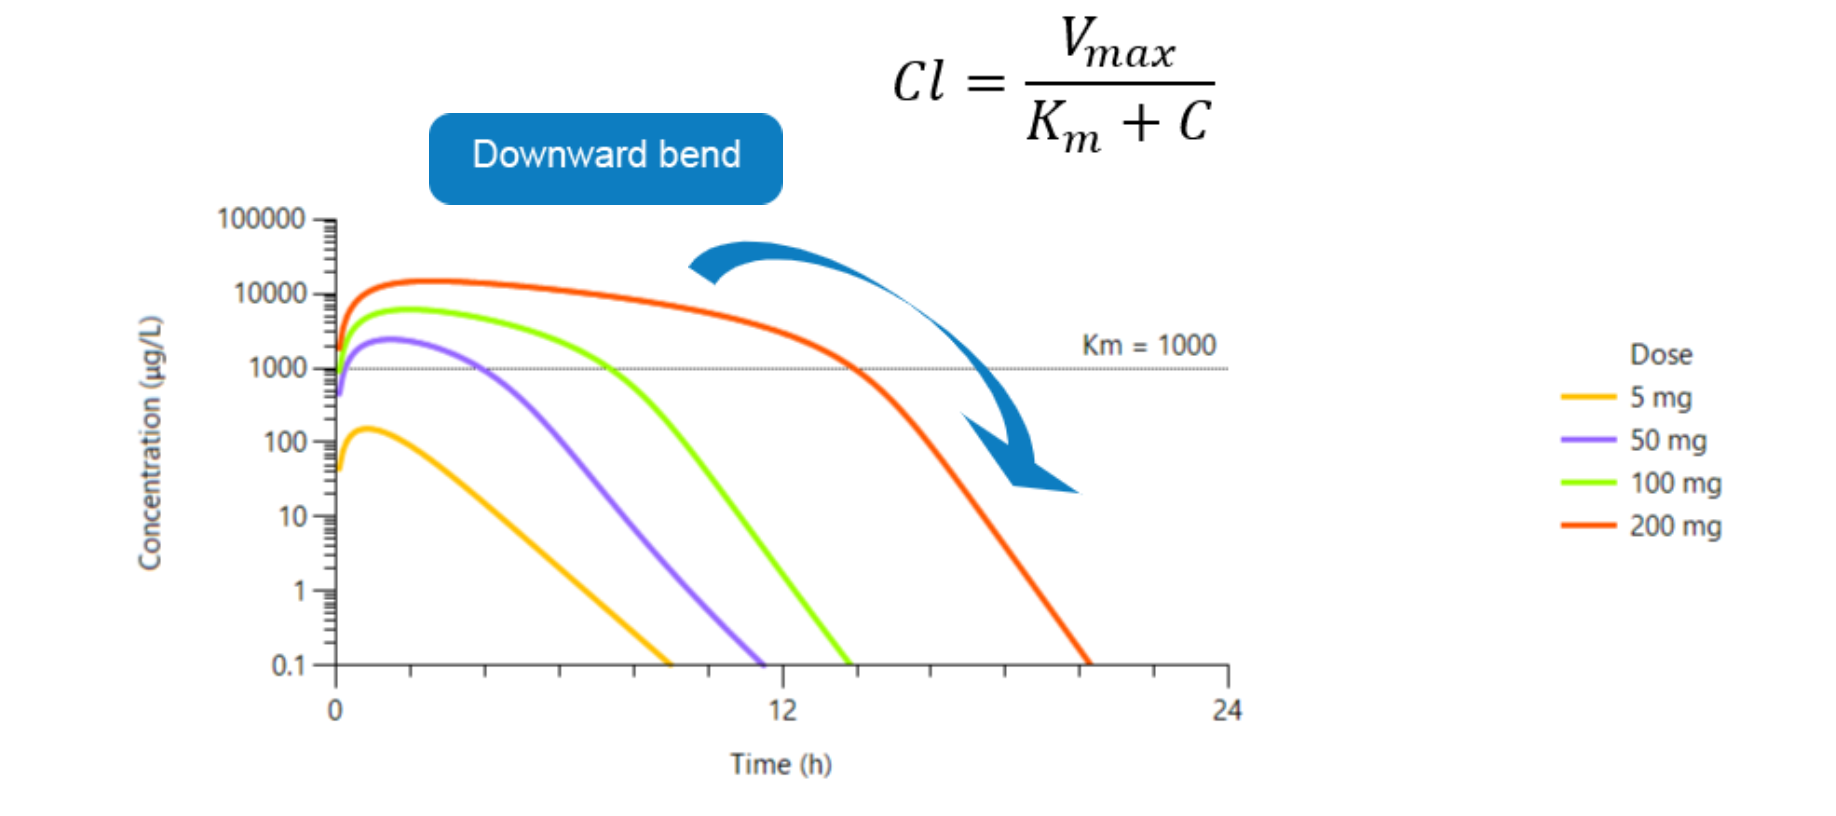
\includegraphics{./img/saturation-2.png} Let's see how this change
  affects the shape of the PK curve click next to continue
  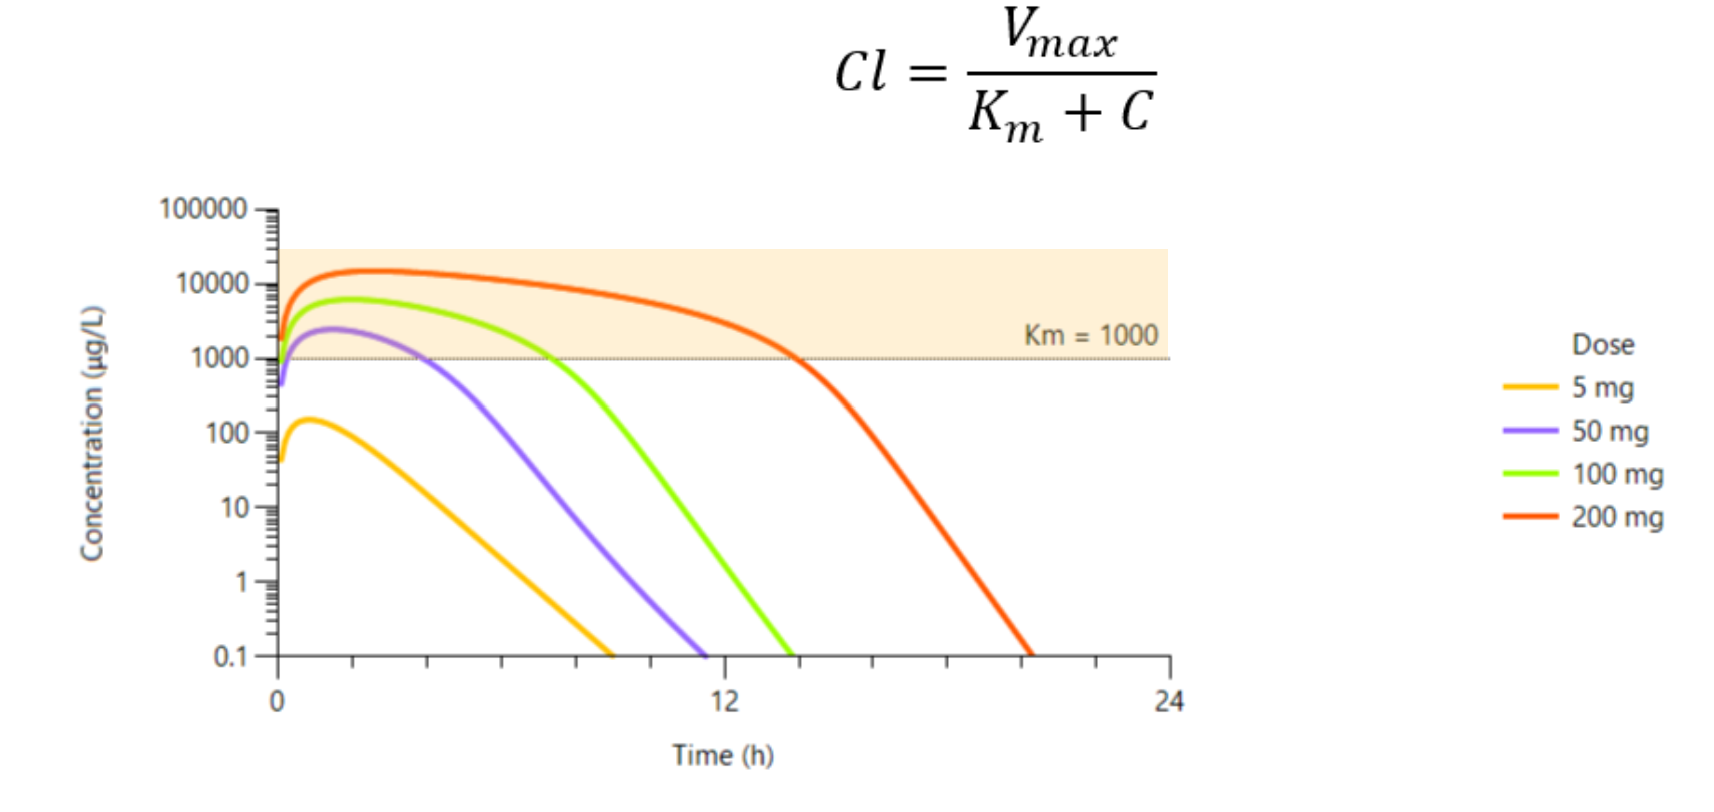
\includegraphics{./img/saturation-3.png} here are simulated curves for
  a drug that has a KM value of 1,000 in a saturating model clearance
  becomes the expression v max over km + c this means that clearance
  depends on the concentration and the clearance is no longer constant
  notice how different doses have PK curves with dramatically different
  shapes notice how many of the curves have a downward bend this
  downward bend is a characteristic of saturating kinetics it may not be
  observed at lower doses but as the dose increases we may encounter
  saturation and it is useful to know what it looks like at the lowest
  dose shown here the yellow curve looks just like a one compartment
  model with linear kinetics as the dose increases we see more
  saturation notice how
\item
  when the concentration is higher than the KM value the apparent
  clearance is much lower and the slopes are much shallower at higher
  concentrations scale
\item
  This breakdown the dose proportionality
\end{itemize}

Linear scale:

\begin{itemize}
\tightlist
\item
  The increase in AUC is far beyond what we would have predicted under
  linear kinetics
\item
  In cases were saturation is observed it is important to have data from
  more than one dose amount so that you can obtain in reliable parameter
  estimates
\end{itemize}

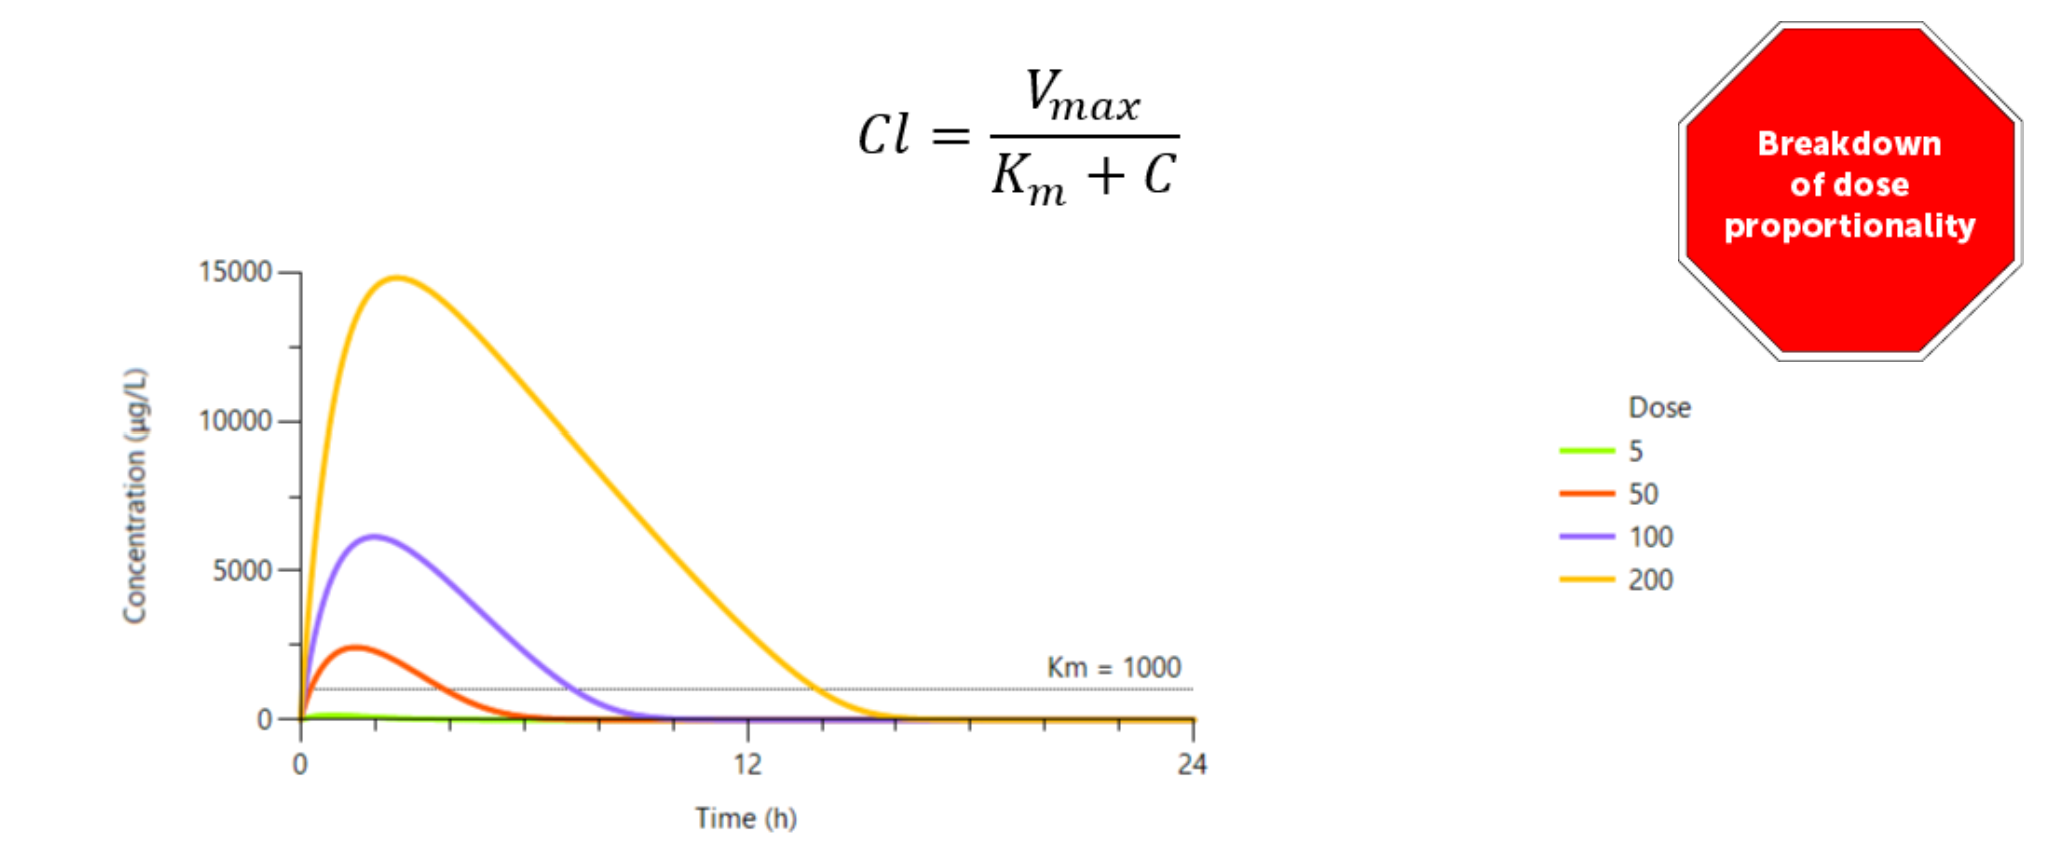
\includegraphics{./img/saturation-4.png}

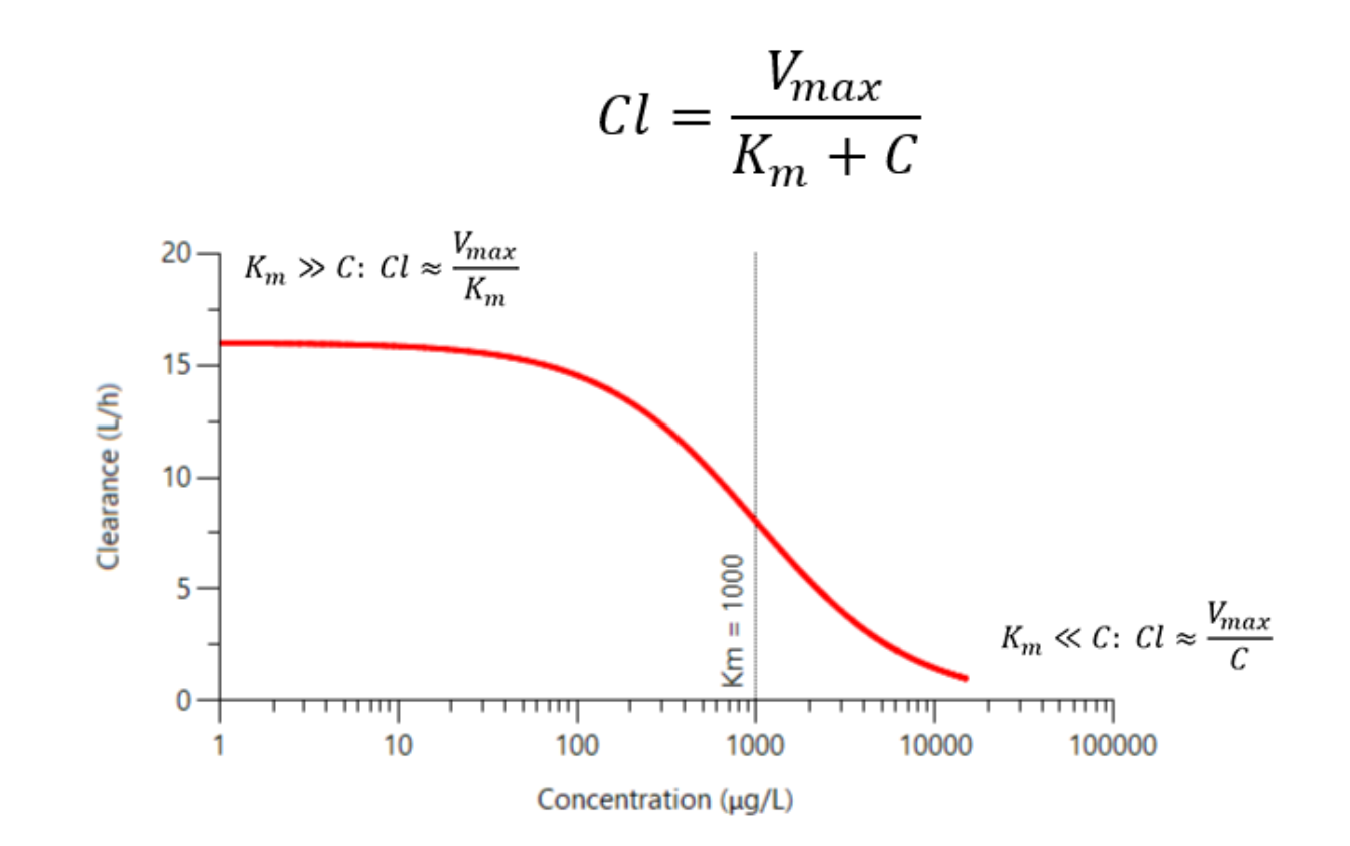
\includegraphics{./img/saturation-5.png} if we consider the expression
for the effective clearance at different concentrations we can consider
two extremes when the concentration is much lower than the KM value we
do not see any saturation and the clearance is constant clearance over
KM at the other extreme when the concentration is much greater than the
KM value The clearance reduces to VMAX over c as the concentration
increases the clearance becomes progressively smaller at very high
concentrations we are overwhelming the elimination pathway usually this
happens when an enzyme has a finite capacity to eliminate the drug and
we are overloading it you may never need to create a model with
saturating elimination but it is good to know when to recognize that
saturation

let's recap the section we have seen that the model structure is
typically defined by the number of compartments the presence or absence
of a time lag and the possibility of saturating elimination These three
items can be combined to make a very large number of potential models
click next to continue

\hypertarget{residual-error}{%
\section{5. residual error}\label{residual-error}}

Residual error:the difference between the observed and predicted
concentrations DV: dependent variable or observed concentration\\
IPRED: Individual prediction, the predicted concentration

\begin{figure}

{\centering 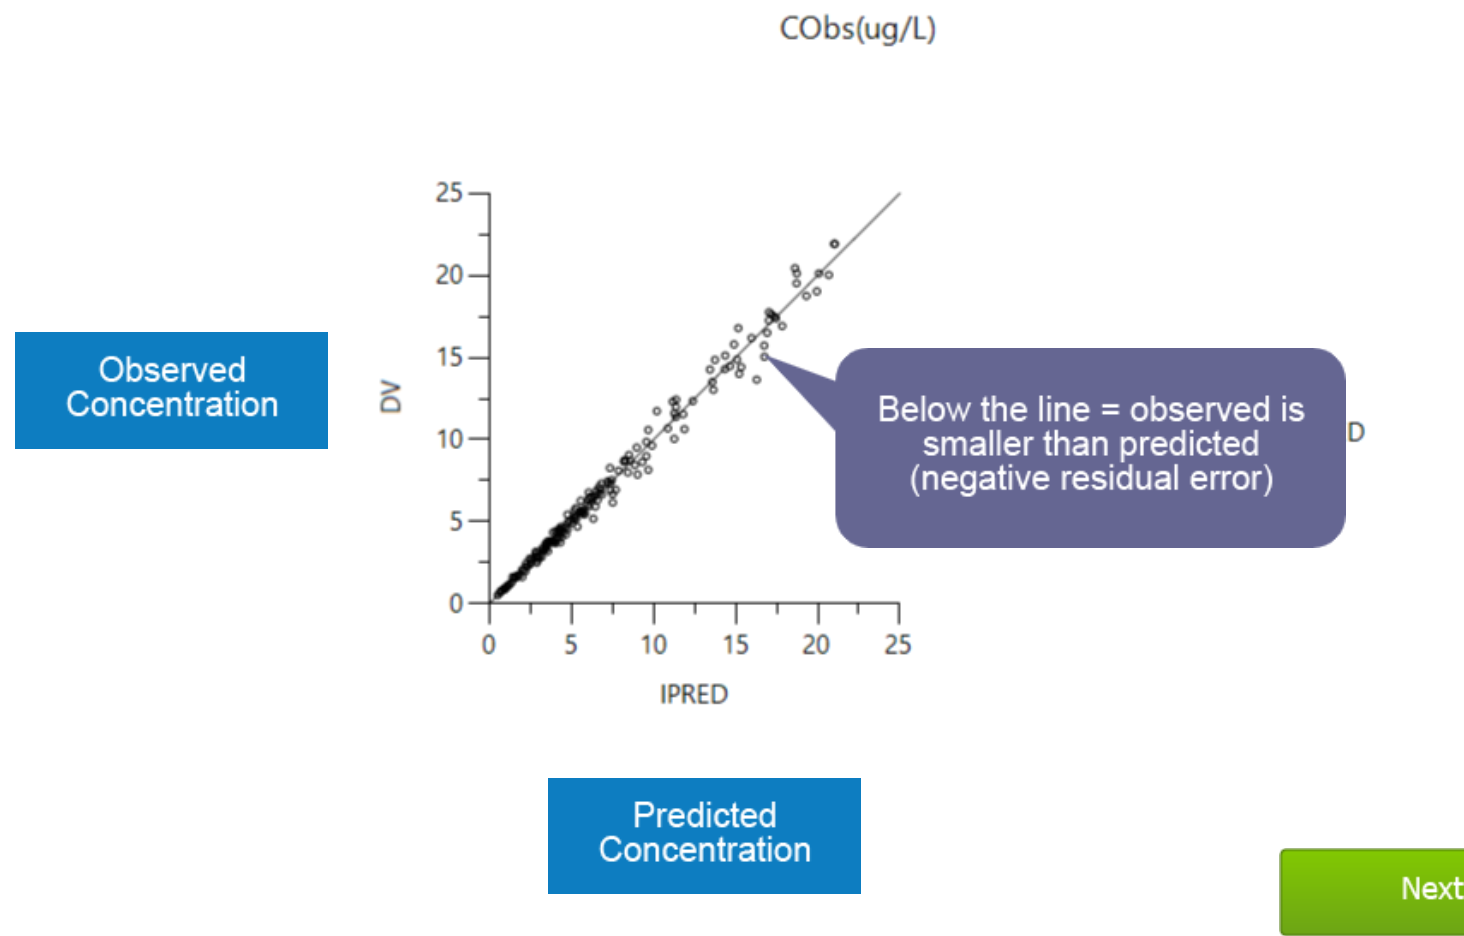
\includegraphics{./img/residual-error-1.png}

}

\caption{resdials}

\end{figure}

ideal prediction would fall on the line positive residual error negative
residual error

Let's look at another type of plot that is more useful for examining the
residuals click next to continue

\begin{itemize}
\tightlist
\item
  These plots show us the residuals on the y-axis with either the
  predicted concentration or the time on the x-axis
\item
  each point is a residual error
\item
  both plots have the same number of points they're just arranged
  differently
\item
  The dotted lines represent two standard deviations in the positive and
  negative directions
\end{itemize}

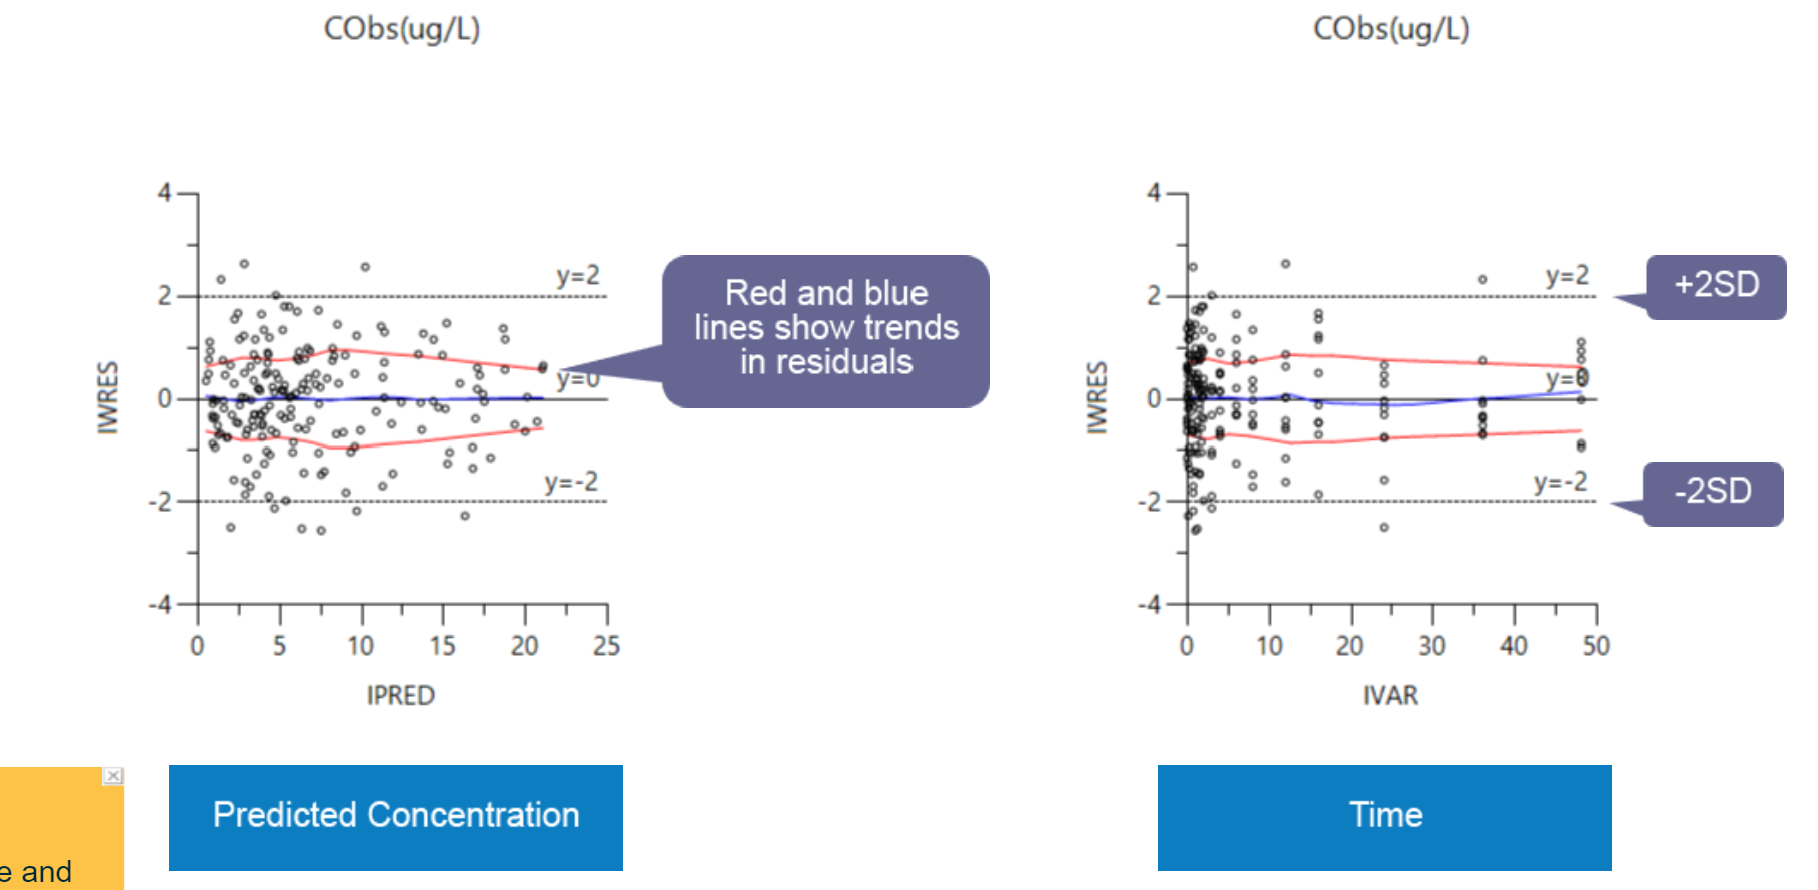
\includegraphics{./img/residual-error-2.png}

Residual worksheet contains the data that was plotted Ires: individual
residual, difference between DV and IPRED

different methods for the residual error - additive : assumes that all
errors are constant regardless of concentration . In practice we usually
find that the error magnitude becomes smaller at smaller concentrations
and therefore additive is not often the best choice - multiplicative,
assumes that the errors are proportional to the concentration of -
additive plus multiplicative: partly constant, partly proportional. at
higher concentrations the error magnitude is proportional but at small
concentrations the error reaches a threshold and does not decrease any
more as the concentration falls

Use multiplicative the initial choice of residual error when building
models

Start your modeling using a multiplicative residual error as you are
optimizing the structural model - after you have decided on the best
structural model then you can start optimizing the residual error model

\bookmarksetup{startatroot}

\hypertarget{summary}{%
\chapter{Summary}\label{summary}}

\hypertarget{pk-model-1}{%
\section{pk model 1}\label{pk-model-1}}

\hypertarget{concentrations-should-be-stacked}{%
\subsection{Concentrations should be
stacked}\label{concentrations-should-be-stacked}}

data format for PK models - observed concentration stacked into a single
column - multiple analytes or metabolites concentration should be its
own column

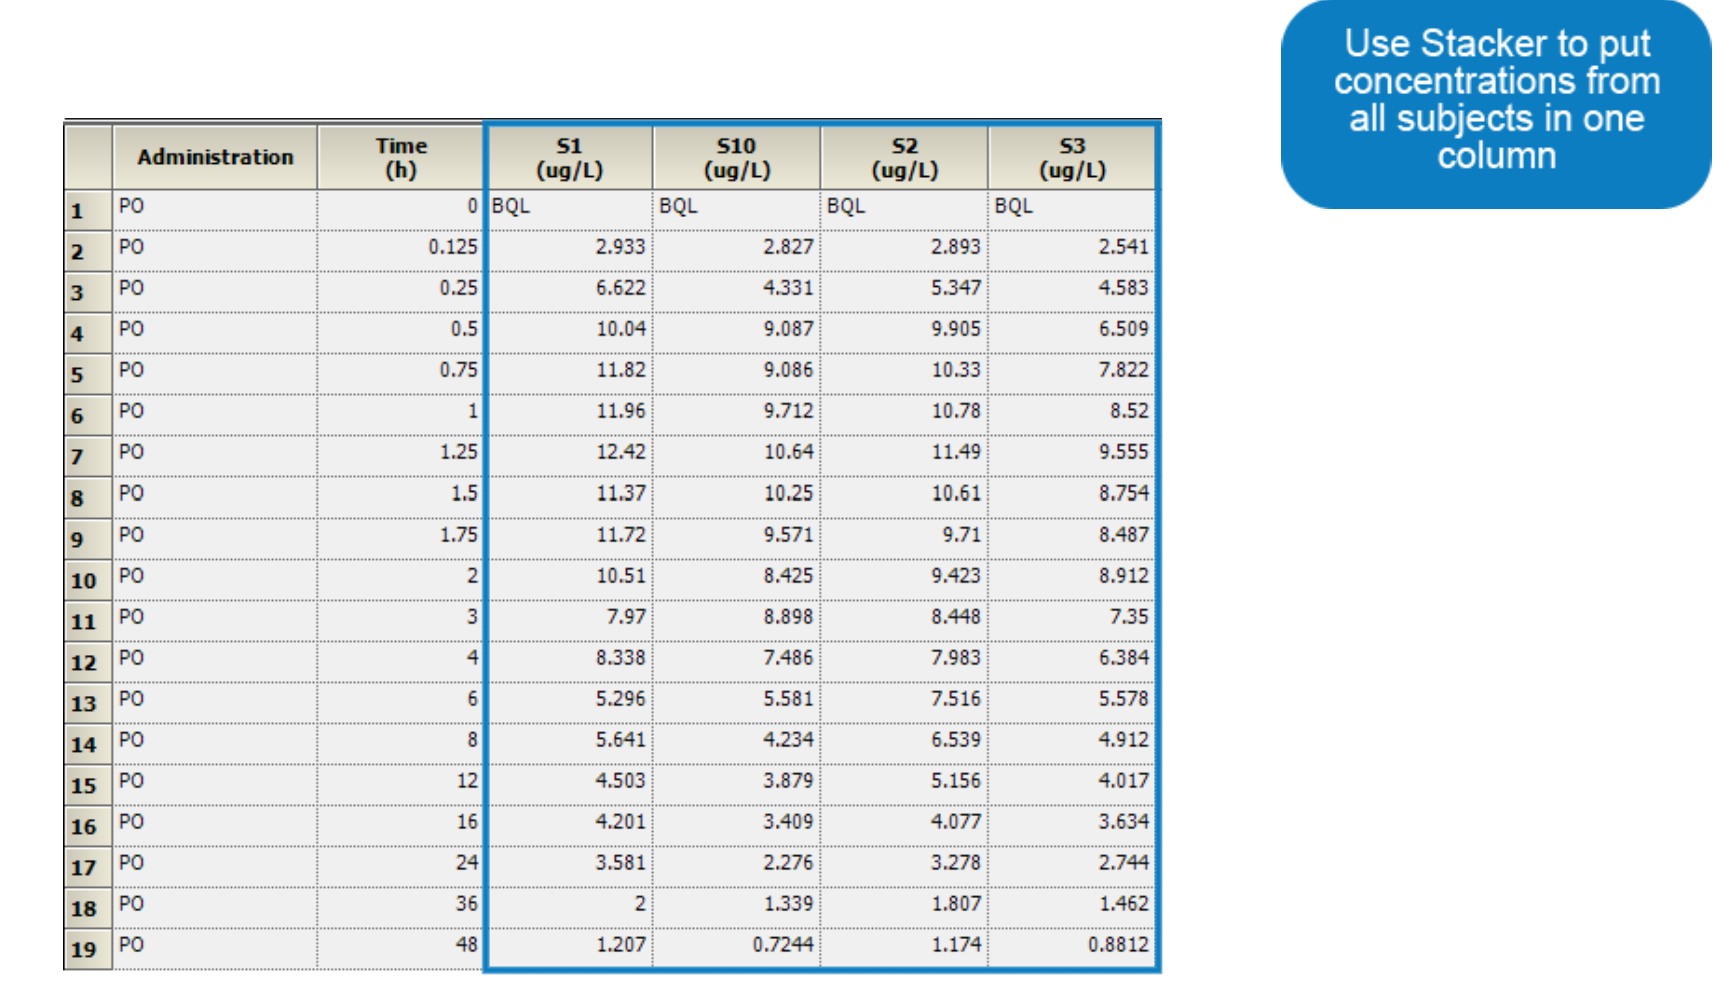
\includegraphics[width=5.60417in,height=\textheight]{./img_model/data-1.png}
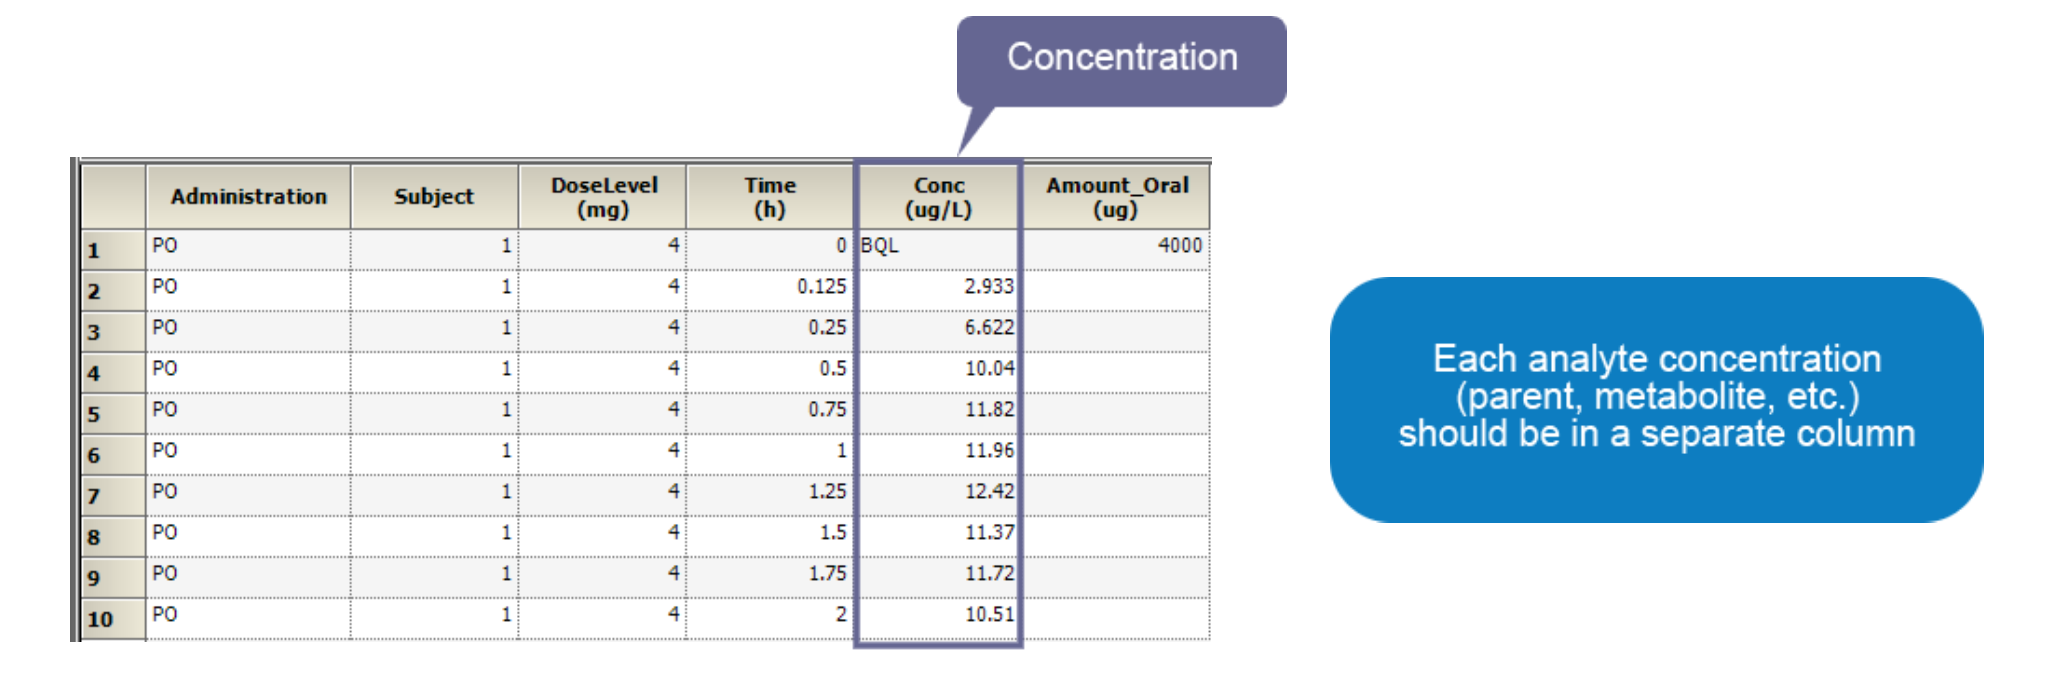
\includegraphics[width=5.59375in,height=2.47917in]{./img_model/data-2.png}

Sort variables

\begin{itemize}
\tightlist
\item
  For multiple PK profiles, one or more sort variables are required.
\item
  Sort variables need to have a value on every row
\item
  In Phoenix text values, blank cells are not a problem
\item
  All non-numeric data is ignored by the model
\end{itemize}

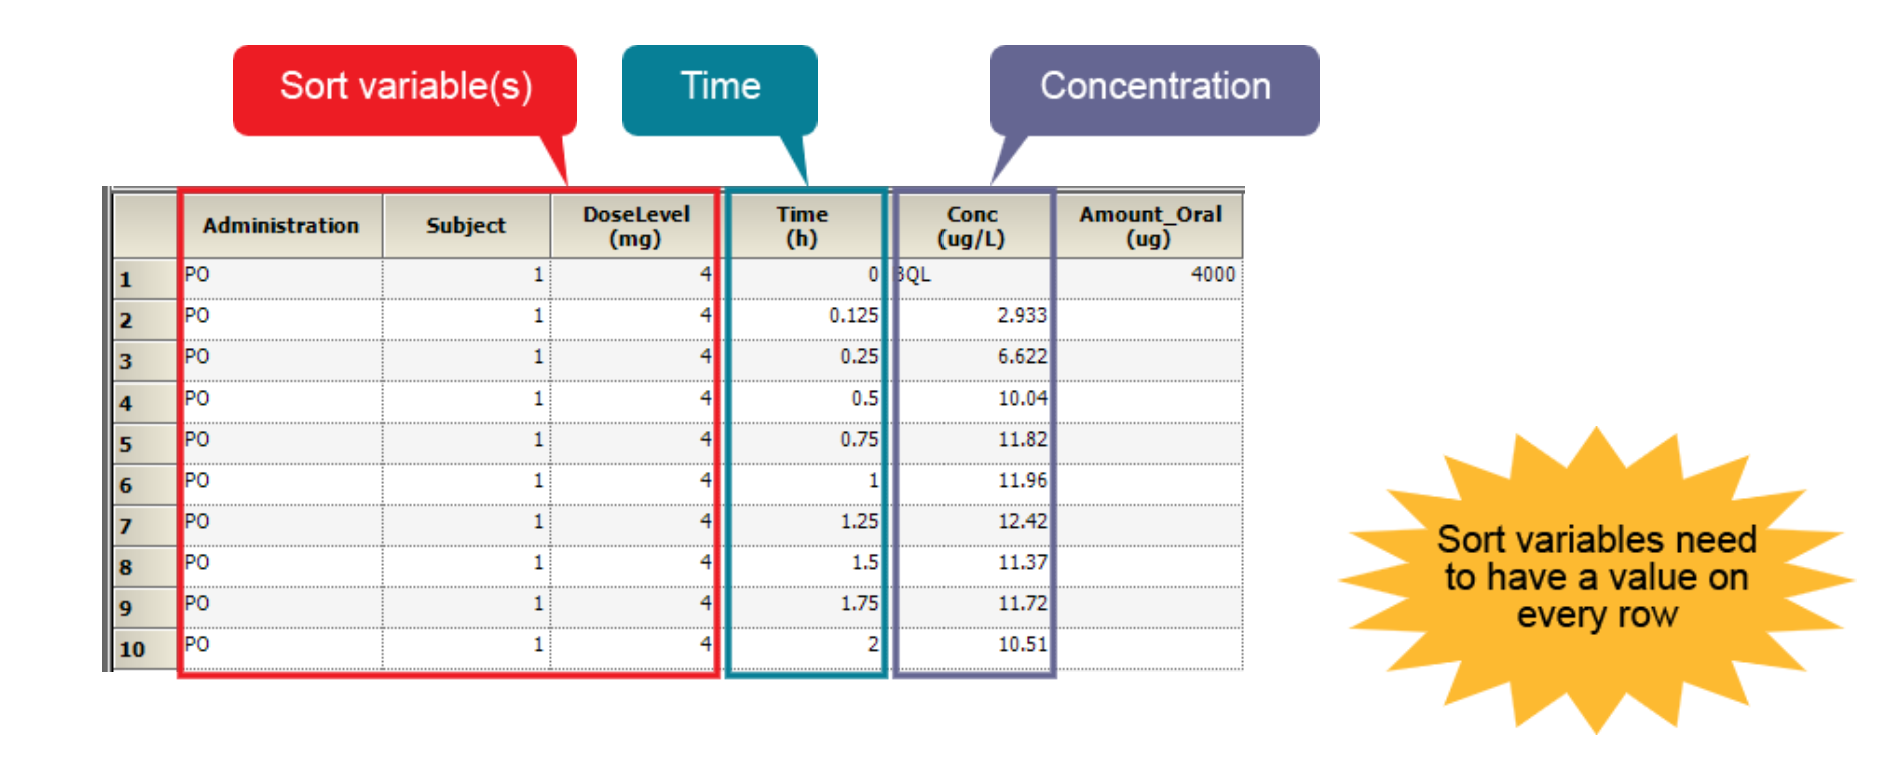
\includegraphics{./img_model/data-3.png}

\begin{itemize}
\tightlist
\item
  amount oral column has a value at time zero and the rest of the rows
  are blank. The dose amount is given only on the row the corresponds to
  a dosing event
\item
  dose level column has a value on every row
\item
  units: unlike NCA the model object does not translate units\\
\item
  The dose unit should always be the same as the unit in the
  concentration
\end{itemize}

And your parameter values keep them the same so that the units will work
out properly One more warning the model object allows you to either map
the dosing amounts in the main input or the dosing input Make sure that
you don't map the dose amount in both places or your administered dose
will be twice as large as you intended click next to continue let's
recap the section we saw how the model object requires stacked
concentrations you should have a single concentration column for each
observation second we use sort variables to define the individual PK
profiles there's nothing wrong with having more sort variables than you
need third we saw how dosing events can be included in the data set
remember that these are entered on the row at the time of the dosing
event and finally we learned that text values and empty cells are okay
in the input and we do not have to do anything to them this completes
the section click

\bookmarksetup{startatroot}

\hypertarget{my-tech-notes}{%
\chapter{My Tech Notes}\label{my-tech-notes}}

\hypertarget{create-a-new-repository-on-the-command-line}{%
\subsection{create a new repository on the command
line}\label{create-a-new-repository-on-the-command-line}}

\begin{verbatim}
echo "# test" >> README.md
git init
git add README.md
git commit -m "first commit"
git branch -M main
git remote add origin https://github.com/drnazmul/test.git
git push -u origin main
\end{verbatim}

\hypertarget{or-push-an-existing-repository-from-the-command-line}{%
\subsection{\ldots or push an existing repository from the command
line}\label{or-push-an-existing-repository-from-the-command-line}}

\begin{verbatim}
git remote add origin https://github.com/drnazmul/test.git
git branch -M main
git push -u origin main
\end{verbatim}

After any change made on github repo but not on the local folder, do the
following

\begin{verbatim}
git pull --rebase origin main
git push origin main
\end{verbatim}

\bookmarksetup{startatroot}

\hypertarget{references}{%
\chapter*{References}\label{references}}
\addcontentsline{toc}{chapter}{References}

\markboth{References}{References}

\hypertarget{refs}{}
\begin{CSLReferences}{1}{0}
\leavevmode\vadjust pre{\hypertarget{ref-alam2006}{}}%
Alam, Muhammad. 2006. {``Geometry of Diffusion and the Performance
Limits of Nanobiosensors.''}

\end{CSLReferences}



\end{document}
